\chapter{Attention as Memory: Sparse, Selective, and Reinterpreted Attention}\label{ch:sparse}

A Transformer already has a memory, and it is a very good one. Every token that passes through
an attention layer leaves behind a key and a value, and every later token can look up any of
them by content. \Cref{ch:foundations} built this mechanism and its key--value (KV) cache, and
\cref{ch:taxonomy} placed it in the survey's taxonomy: the KV cache is \emph{implicit} memory
(a by-product of the forward pass), it is written \emph{online} (one entry per token, at
inference time), and it is \emph{short-term} (it lives only as long as the context)
\citep{zhoubian2026memory}. Its weakness is cost. A query must compare itself with every stored
key, so prefilling $T$ tokens costs $\bigO(T^2)$ work, and the cache itself grows linearly with
$T$ and must be read in full at every decoding step.

This chapter studies the systems that keep the attention-style memory but control how it is
used. The survey (its Section III-B) describes this family as introducing \emph{admission},
\emph{access} and \emph{retention} control over an online memory: which tokens may enter the
store, which stored entries a query may read, and which entries are kept in exact form rather
than evicted or summarized. We first build the background from scratch: attention as
content-addressable memory, the log-sum-exp algebra that lets us split attention into pieces,
sliding windows and attention sinks, fixed sparse patterns, and selective attention
(\cref{sec:c04-background}). We then study four 2025--2026 systems in depth:
\begin{itemize}
  \item \textbf{MoBA} (\cref{sec:c04-moba}) routes each query to a few blocks of the KV cache
  with a parameter-free top-$k$ gate, applying mixture-of-experts routing to memory access.
  \item \textbf{NSA} (\cref{sec:c04-nsa}) combines three learned views of the context, namely
  compressed block summaries, a few selected fine-grained blocks and a sliding window, and
  designs the selection so that GPU kernels can exploit it.
  \item \textbf{RATTENTION} (\cref{sec:c04-rattention}) keeps an exact sliding window and folds
  every token that leaves the window into a linear-attention state, and asks how small the
  window can be.
  \item \textbf{HyperMLP} (\cref{sec:c04-hypermlp}) does not sparsify attention at all. It
  reinterprets an attention head as a two-layer MLP whose hidden layer has one unit per past
  token, and replaces the softmax with ReLU or GLU selection.
\end{itemize}
We close with a comparison (\cref{sec:c04-comparison}). Linear attention, which RATTENTION
uses as its long-range memory, is developed in \cref{ch:linear}; here we only need its
recurrent and chunkwise forms.

% =====================================================================================
\section{Background: attention as a content-addressable memory}\label{sec:c04-background}

\subsection{Reading from the KV cache}\label{sec:c04-cam}

Fix one attention head. At time $t$ the head has stored the pairs $(\vk_s,\vv_s)$ for
$s=1,\dots,t$, with $\vk_s\in\R^{d_k}$ and $\vv_s\in\R^{d_v}$. A query $\vq_t\in\R^{d_k}$ reads
from this store in three steps:
\begin{align}
  z_{ts} &= \frac{\vq_t\T\vk_s}{\sqrt{d_k}}, \qquad s = 1,\dots,t, \label{eq:c04-scores}\\
  a_{ts} &= \frac{\exp(z_{ts})}{\sum_{s'=1}^{t}\exp(z_{ts'})}, \label{eq:c04-weights}\\
  \vo_t  &= \sum_{s=1}^{t} a_{ts}\,\vv_s. \label{eq:c04-read}
\end{align}
Stacking all queries as rows of $\mQ$ (and likewise $\mK$, $\mV$) gives the familiar matrix form
$\mO = \softmax(\mQ\mK\T/\sqrt{d_k} + \mM)\mV$, where the causal mask $\mM$ has $0$ on and
below the diagonal and $-\infty$ above it, so that $\exp(-\infty)=0$ removes future positions.

\begin{definition}[Attention as a content-addressable memory]\label{def:c04-cam}
The \emph{memory} of a head at time $t$ is the set $\mathcal{M}_t=\{(\vk_s,\vv_s)\}_{s\le t}$.
\emph{Writing} appends one pair per token. \emph{Reading} with a query $\vq$ returns the
convex combination \eqref{eq:c04-read} of stored values, weighted by how well $\vq$ matches
each stored key.
\end{definition}

The word ``content-addressable'' means that entries are found by \emph{what they contain} (the
match $\vq\T\vk_s$), not by \emph{where they are} (an index $s$). Three properties of this
memory matter for the whole chapter:
\begin{enumerate}
  \item \textbf{Lossless, append-only writes.} Nothing is ever overwritten or forgotten while
  the token stays in the context. This is why attention is so good at exact recall, and why
  the survey calls it the canonical form of implicit memory.
  \item \textbf{Soft reads.} Every stored entry receives a positive weight $a_{ts}>0$, however
  irrelevant. The weights sum to one, so entries compete for a fixed budget of probability
  mass.
  \item \textbf{Linear growth.} Per layer and per key--value head the store holds
  $t(d_k+d_v)$ numbers, and a read touches all of them.
\end{enumerate}

\begin{example}[A read with $d_k=d_v=2$]\label{ex:c04-read}
Store four entries with keys $\vk_1=(1,0)$, $\vk_2=(0,1)$, $\vk_3=(-1,0)$, $\vk_4=(1,1)$ and
values $\vv_1=(1,0)$, $\vv_2=(0,1)$, $\vv_3=(-1,-1)$, $\vv_4=(2,2)$. Query with
$\vq=(2,1)$. The scaled scores are $\vz=(2,1,-2,3)/\sqrt2\approx(1.414,\,0.707,\,-1.414,\,2.121)$.
Exponentiating and normalizing gives $\va\approx(0.279,\,0.138,\,0.017,\,0.566)$, and the read is
$\vo\approx 0.279\,\vv_1+0.138\,\vv_2+0.017\,\vv_3+0.566\,\vv_4\approx(1.396,\,1.254)$. More than
half of the mass sits on one entry and the entry $\vk_3$, which points away from the query,
gets less than 2\%. Real attention distributions are often even more concentrated. This is
the observation that sparse attention exploits: if most of the mass sits on a few entries,
reading only those entries changes the output very little.
\end{example}

\subsection{What exact attention costs}\label{sec:c04-costs}

Count multiply--adds for one head. Computing all scores $\mQ\mK\T$ for a causal prefix of
length $T$ needs about $\tfrac12T^2d_k$ multiply--adds, and the weighted sum $\mA\mV$ about
$\tfrac12T^2d_v$; prefill is therefore $\bigO(T^2 d_k)$. In decoding, token $t$ needs
$\bigO(t\,d_k)$ work, but the real bottleneck is memory traffic: the whole cache of
$t(d_k+d_v)$ numbers per key--value head must be read from GPU memory for every generated
token (\cref{ch:foundations}). Summed over layers, a model with $L$ layers and $H_{kv}$
key--value heads stores $2LH_{kv}d_k$ numbers per token (taking $d_v=d_k$).

A sparse attention method replaces the full index set $\{1,\dots,t\}$ in
\eqref{eq:c04-weights}--\eqref{eq:c04-read} by a subset $\mathcal{I}_t$ of size $N_t$:
\begin{equation}\label{eq:c04-sparse-read}
  \vo_t = \sum_{s\in\mathcal{I}_t} \frac{\exp(z_{ts})}{\sum_{s'\in\mathcal{I}_t}\exp(z_{ts'})}\,\vv_s .
\end{equation}
The read now costs $\bigO(N_t d_k)$ instead of $\bigO(t d_k)$. Two different savings are
possible, and it is important to keep them apart:
\begin{itemize}
  \item \textbf{Access sparsity}: the full cache is kept, but each query reads only
  $\mathcal{I}_t$. Compute and memory traffic per query shrink; the memory footprint does not.
  MoBA and NSA are of this kind.
  \item \textbf{Retention sparsity}: entries outside some set are deleted (or summarized), so the
  footprint itself is bounded. Sliding windows and StreamingLLM are of this kind, and
  RATTENTION's local layers are too.
\end{itemize}

\subsection{Splitting attention into pieces: the log-sum-exp merge}\label{sec:c04-lse}

Almost every efficient attention kernel, including FlashAttention
\citep{c01-dao2022flashattention,c01-dao2024flashattention2} (\cref{ch:foundations}) and the
MoBA and NSA implementations below, computes attention over pieces of the key set and merges
the pieces afterwards. The merge is exact, and we now derive it because both MoBA's forward
and its backward pass depend on it.

For a query $\vq$ and a key set $\mathcal{I}$ define the \emph{log-sum-exp} (LSE) and the
partial output
\begin{equation}\label{eq:c04-lse}
  \lambda(\mathcal{I}) = \log\sum_{s\in\mathcal{I}} e^{z_s}, \qquad
  \vo(\mathcal{I}) = \sum_{s\in\mathcal{I}} e^{z_s-\lambda(\mathcal{I})}\,\vv_s .
\end{equation}

\begin{proposition}[Exact merge]\label{prop:c04-merge}
Let $\mathcal{I}=\mathcal{I}_1\cup\mathcal{I}_2$ with $\mathcal{I}_1\cap\mathcal{I}_2=\emptyset$
and write $\lambda_j=\lambda(\mathcal{I}_j)$, $\vo_j=\vo(\mathcal{I}_j)$. Then
\begin{equation}\label{eq:c04-merge}
  \lambda(\mathcal{I}) = \log\!\left(e^{\lambda_1}+e^{\lambda_2}\right), \qquad
  \vo(\mathcal{I}) = e^{\lambda_1-\lambda(\mathcal{I})}\,\vo_1 + e^{\lambda_2-\lambda(\mathcal{I})}\,\vo_2 .
\end{equation}
\end{proposition}
\begin{proof}
Because the sets are disjoint, $\sum_{s\in\mathcal{I}}e^{z_s}=\sum_{s\in\mathcal{I}_1}e^{z_s}
+\sum_{s\in\mathcal{I}_2}e^{z_s}=e^{\lambda_1}+e^{\lambda_2}$; take logarithms. For the output,
$\sum_{s\in\mathcal{I}_j}e^{z_s}\vv_s=e^{\lambda_j}\vo_j$ by definition \eqref{eq:c04-lse}, so
$\vo(\mathcal{I})=e^{-\lambda(\mathcal{I})}(e^{\lambda_1}\vo_1+e^{\lambda_2}\vo_2)$.
\end{proof}

In floating point one subtracts $m=\max(\lambda_1,\lambda_2)$ before exponentiating:
$\lambda(\mathcal{I})=m+\log(e^{\lambda_1-m}+e^{\lambda_2-m})$, so that no exponential exceeds
one \citep{c01-milakov2018online}. The merge extends to any number of pieces by induction.

The backward pass has an equally useful property. Let $\loss$ depend on $\vo=\vo(\mathcal{I})$
and write $\bar{\vo}=\partial\loss/\partial\vo$.

\begin{proposition}[Piecewise backward]\label{prop:c04-merge-bwd}
With $a_s=e^{z_s-\lambda(\mathcal{I})}$ the final attention weights,
\begin{equation}\label{eq:c04-merge-bwd}
  \frac{\partial\loss}{\partial z_s} = a_s\left(\bar{\vo}\T\vv_s - \bar{\vo}\T\vo\right)
  \qquad\text{for every } s\in\mathcal{I}.
\end{equation}
Hence the gradient for the scores of piece $\mathcal{I}_j$ can be computed from piece $j$'s own
keys and values plus two \emph{global} quantities: the merged LSE $\lambda(\mathcal{I})$ and the
merged output $\vo$.
\end{proposition}
\begin{proof}
$\vo=\sum_r a_r\vv_r$ and the softmax Jacobian is $\partial a_r/\partial z_s=a_r(\delta_{rs}-a_s)$.
Then $\partial\loss/\partial z_s=\sum_r\bar{\vo}\T\vv_r\,a_r(\delta_{rs}-a_s)
=a_s\bar{\vo}\T\vv_s-a_s\sum_ra_r\bar{\vo}\T\vv_r=a_s(\bar{\vo}\T\vv_s-\bar{\vo}\T\vo)$.
\end{proof}

FlashAttention's backward kernel takes exactly these inputs (queries, the piece's keys and
values, the output, the LSE and $\bar{\vo}$) and evaluates \eqref{eq:c04-merge-bwd}, so one
can call it once per piece with the global LSE and output. We checked
\eqref{eq:c04-merge-bwd} against finite differences in NumPy (agreement to $10^{-10}$).

\begin{lstlisting}[caption={Reference implementation (ours): merging two attention pieces by log-sum-exp.},label={lst:c04-merge}]
def merge(o1, lse1, o2, lse2):
    # o1, o2: [N, d_v] partial outputs; lse1, lse2: [N] their log-sum-exps
    m = torch.maximum(lse1, lse2)                  # stabiliser
    lse = m + torch.log(torch.exp(lse1 - m) + torch.exp(lse2 - m))
    o = torch.exp(lse1 - lse)[:, None] * o1 + torch.exp(lse2 - lse)[:, None] * o2
    return o, lse
\end{lstlisting}

\subsection{Sliding windows, attention sinks and StreamingLLM}\label{sec:c04-streaming}

The simplest retention policy keeps only the most recent tokens. \emph{Sliding-window attention}
(SWA) with window $w$ uses
\begin{equation}\label{eq:c04-swa}
  \mathcal{I}^{\mathrm{win}}_t = \{\max(1,t-w),\dots,t\},
\end{equation}
that is, the current token and $w$ tokens to its left (implementations differ by one in what
they call the window size; we use this convention throughout and point out where code differs).
Memory per head is $\bigO(w)$ and the cost per query is $\bigO(w d_k)$, independent of $t$.
Information older than $w$ tokens is not lost from the network entirely: after $L$ stacked
windowed layers a token can influence positions up to $Lw$ away, because each layer can relay
information one window further. But the relay is lossy, and a single layer can no longer look
up an old fact directly.

Naive windowing has a surprising failure mode. \citet{xiao2023streamingllm} observed that
pretrained models put a large share of attention weight on the first few tokens of the sequence,
regardless of their content. They called these tokens \emph{attention sinks}. A plausible reason
is the sum-to-one constraint in \eqref{eq:c04-weights}: when a head has nothing useful to read,
it must still place its probability mass somewhere, and the always-visible first tokens become
the default. Once the window slides past them, that mass is redistributed over the remaining
tokens and the model's outputs degrade sharply. StreamingLLM's fix is to keep a handful of sink
tokens forever in addition to the recent window,
\begin{equation}\label{eq:c04-sink}
  \mathcal{I}^{\mathrm{sink}}_t = \{1,\dots,n_{\mathrm{sink}}\}\cup\mathcal{I}^{\mathrm{win}}_t,
\end{equation}
which lets a model trained with full attention generate over very long streams with a bounded
cache and without retraining. In the survey's vocabulary this is an \emph{eviction policy}: most
past states are continuously evicted, a few anchors are retained (survey Table II lists
StreamingLLM under ``admission, eviction, and consolidation'').

\subsection{Fixed sparse patterns}\label{sec:c04-fixed}

Early sparse attention mostly used patterns fixed in advance. The \emph{Sparse Transformer}
of \citet{child2019sparse} factorizes attention into a local component (the previous few
positions) and a strided component (every $m$-th earlier position). With
$m\approx\sqrt{T}$, each query reads $\bigO(\sqrt T)$ keys and the whole layer costs
$\bigO(T\sqrt T)$, while any two positions are connected through at most two hops.
\emph{Longformer} \citep{beltagy2020longformer} uses a sliding window (optionally dilated, with
gaps) plus a few task-chosen \emph{global} tokens that attend to and are attended by every
position. \emph{BigBird} \citep{zaheer2020bigbird} combines windowed, global and random
attention, and proves that such patterns keep the expressive power of full attention.
\Cref{fig:c04-patterns} draws some of these patterns as masks.

\begin{figure}[t]
\centering
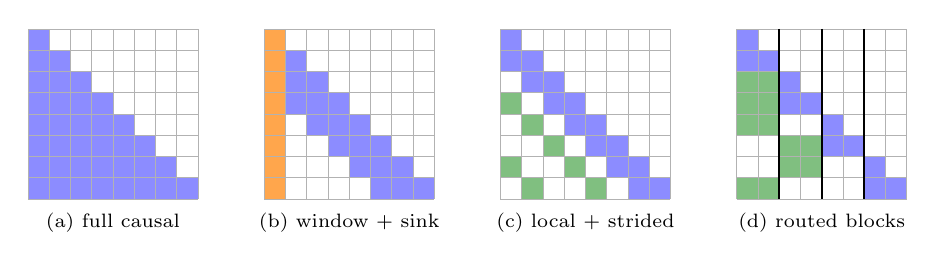
\begin{tikzpicture}[x=0.27cm,y=0.27cm]
  % (a) full causal
  \begin{scope}
    \foreach \i in {0,...,7}{\foreach \j in {0,...,\i}{\fill[blue!45] (\j,-\i) rectangle ++(1,-1);}}
    \draw[step=1,gray!60,very thin] (0,-8) grid (8,0);
    \node[below] at (4,-8.2) {\scriptsize (a) full causal};
  \end{scope}
  % (b) window + sink
  \begin{scope}[xshift=3.0cm]
    \foreach \i in {0,...,7}{
      \pgfmathtruncatemacro{\lo}{max(0,\i-2)}
      \foreach \j in {\lo,...,\i}{\fill[blue!45] (\j,-\i) rectangle ++(1,-1);}
      \fill[orange!70] (0,-\i) rectangle ++(1,-1);}
    \draw[step=1,gray!60,very thin] (0,-8) grid (8,0);
    \node[below] at (4,-8.2) {\scriptsize (b) window $+$ sink};
  \end{scope}
  % (c) local + strided
  \begin{scope}[xshift=6.0cm]
    \foreach \i in {0,...,7}{
      \foreach \j in {0,...,\i}{
        \pgfmathtruncatemacro{\r}{mod(\i-\j,3)}
        \ifnum\r=0 \fill[green!50!black!50] (\j,-\i) rectangle ++(1,-1);\fi}
      \pgfmathtruncatemacro{\lo}{max(0,\i-1)}
      \foreach \j in {\lo,...,\i}{\fill[blue!45] (\j,-\i) rectangle ++(1,-1);}}
    \draw[step=1,gray!60,very thin] (0,-8) grid (8,0);
    \node[below] at (4,-8.2) {\scriptsize (c) local $+$ strided};
  \end{scope}
  % (d) MoBA-style block routing
  \begin{scope}[xshift=9.0cm]
    \foreach \i/\h in {2/0,3/0,4/0,5/1,6/1,7/0}{\fill[green!50!black!50] (2*\h,-\i) rectangle ++(2,-1);}
    \foreach \i in {0,...,7}{
      \pgfmathtruncatemacro{\lo}{2*floor(\i/2)}
      \foreach \j in {\lo,...,\i}{\fill[blue!45] (\j,-\i) rectangle ++(1,-1);}}
    \draw[step=1,gray!60,very thin] (0,-8) grid (8,0);
    \foreach \x in {2,4,6}{\draw[black,thick] (\x,0) -- (\x,-8);}
    \node[below] at (4,-8.2) {\scriptsize (d) routed blocks};
  \end{scope}
\end{tikzpicture}
\caption{Attention masks for $T=8$ (row $=$ query, column $=$ key; filled $=$ read).
(a) Full causal attention. (b) A window of the current and two previous tokens plus one sink
token (orange). (c) A local window plus every third earlier position, as in the Sparse
Transformer's strided pattern. (d) Content-routed blocks of size $B=2$: each query reads its own
block causally (blue) plus one earlier block chosen by a gate (green), as in MoBA with $k=2$.
Patterns (b) and (c) are fixed in advance; (d) depends on the content.}
\label{fig:c04-patterns}
\end{figure}

All of these patterns decide \emph{where} to look before seeing \emph{what} is there. That is
their strength (they are cheap and kernel-friendly) and their weakness: a fact that falls outside
the pattern is invisible to a single layer, however relevant it is.

\subsection{Selective attention}\label{sec:c04-selective}

\citet{leviathan2024selective} observe that some context tokens will never be needed again (a
variable that has been overwritten, say). \emph{Selective attention} is a parameter-free change
to attention that lets earlier tokens be \emph{down-weighted for all future queries} once some
token has decided they are no longer needed. One way to formalize this is to compute a
non-negative selection matrix $\mP$ from the attention logits of one designated head (for
example $P_{ij}=\ReLU(z_{ij})$ for $j<i$, with the first token exempt), accumulate it over
queries, $F_{ij}=\sum_{i'<i}P_{i'j}$, and subtract the accumulated penalty from the logits of
all heads, $z_{ij}\leftarrow z_{ij}-F_{ij}$; the paper's exact parameterization may differ. A
token whose penalty has grown large contributes almost nothing to later reads, so it can be
pruned from the context buffer, which reduces inference memory and compute. In the survey's
terms, selective attention is an implicit \emph{admission} control: every token is still
written, but the model learns which ones remain worth reading.

\subsection{The memory view: admission, access and retention}\label{sec:c04-memoryview}

The survey's Section III-B proposes a single lens for this whole family. Standard attention
treats all past tokens as equally admissible memory entries; sparse, selective and structured
attention impose control on the online memory. We make the three controls precise.

\begin{definition}[Admission, access and retention]\label{def:c04-controls}
For a query at time $t$:
\begin{itemize}
  \item the \emph{retained set} $\mathcal{R}_t\subseteq\{1,\dots,t\}$ contains the tokens whose
  exact key--value pairs are still stored, possibly together with \emph{summaries} of evicted
  tokens (compressed keys, a recurrent state);
  \item the \emph{access set} $\mathcal{I}_t\subseteq\mathcal{R}_t$ contains the entries that
  the query actually reads in \eqref{eq:c04-sparse-read};
  \item \emph{admission} decides how strongly a newly written entry can influence later reads
  (selective attention's penalty, or a gate in front of a branch).
\end{itemize}
\end{definition}

Fixed patterns choose $\mathcal{I}_t$ by position; content-routed methods (MoBA, NSA) choose it
by content; windowed methods (SWA, StreamingLLM, RATTENTION's local branch) shrink
$\mathcal{R}_t$ itself; summaries (NSA's compressed tokens, RATTENTION's linear state) give a
coarse view of what was evicted or skipped. Note that none of these mechanisms adds an explicit
read/write interface: the controls are embedded in the attention pattern, so in the survey's
taxonomy all of them remain \emph{implicit}, \emph{online}, \emph{short-term} memory. The survey
summarizes the family by saying that such mechanisms do not scale by storing more, but by
carefully controlling how information is admitted, accessed and retained within the forward
computation.

% =====================================================================================
\section{MoBA: Mixture of Block Attention}\label{sec:c04-moba}

\subsection{Motivation}

Fixed patterns impose what the MoBA authors call strong structure: a window assumes that recent
tokens matter, a sink assumes that the first tokens matter, a stride assumes a periodic
dependency. Each assumption suits some tasks and fails on others. The alternative used in
\cref{ch:linear}, replacing softmax attention by a recurrent state, changes the memory itself and
usually requires training a model from scratch. MoBA \citep{lu2025moba} follows a ``less
structure'' principle instead: keep softmax attention and the whole KV cache, but let \emph{each
query decide} which parts of the cache to read.

The decision borrows from mixture-of-experts (MoE) layers \citep{c01-shazeer2017moe},
where a router sends each token to its top-$k$ experts (\cref{ch:lookup}). MoBA cuts the context
into blocks, treats each block as an ``expert'', and routes each query to its top-$k$ blocks. Two
choices make this practical. First, the router has \emph{no parameters}: it scores blocks with
the same queries and keys that attention already computes. Second, MoBA reduces exactly to full
attention when $k$ covers all blocks, so a layer can be switched between MoBA and full attention
at any point of training or inference. The repository README stresses one limitation up front:
MoBA needs continued training of an existing model to obtain its benefits; it is not a drop-in
replacement for an unmodified pretrained model.

\begin{taxonomy}
\textbf{Representation:} implicit (the ordinary KV cache).
\textbf{Update dynamics:} online (one key--value pair is appended per token).
\textbf{Persistence:} short-term; Table I of \citet{zhoubian2026memory} lists MoBA as online,
short-term, ``content-routed sparse KV blocks''.
\textbf{Update rule:} the write is the usual append; what MoBA changes is the \emph{read}. The
survey (Section III-B) calls this content-routed sparse attention: block-level memory access
by MoE-style routing, i.e.\ adaptive \emph{access} control rather than a new storage substrate.
\end{taxonomy}

\subsection{Formulation}

\paragraph{Blocks and block keys.}
Split the positions $1,\dots,T$ into $n=\lceil T/B\rceil$ consecutive blocks
$\mathcal{B}_i=\{(i-1)B+1,\dots,\min(iB,T)\}$ and write $b(t)=\lceil t/B\rceil$ for the block
that contains position $t$. Each block is summarized by the mean of its keys,
\begin{equation}\label{eq:c04-moba-kbar}
  \bar\vk_i = \frac{1}{\abs{\mathcal{B}_i}}\sum_{s\in\mathcal{B}_i}\vk_s .
\end{equation}

\paragraph{Gate.}
The affinity of query $t$ for block $i$ is $r_{ti}=\vq_t\T\bar\vk_i$. Causality imposes two
rules, and the top-$k$ gate is applied to what remains:
\begin{equation}\label{eq:c04-moba-gate}
  g_{ti} = \begin{cases}
    1 & i = b(t) \quad\text{(current block: always read)},\\
    0 & i > b(t) \quad\text{(future block: never read)},\\
    1 & i < b(t) \text{ and } r_{ti}\in\TopK\big(\{r_{tj}: j<b(t)\},\,k-1\big),\\
    0 & \text{otherwise}.
  \end{cases}
\end{equation}
So $k$ counts the current block: each query reads its own block plus the $k-1$ most affine
earlier blocks (or all earlier blocks if there are fewer than $k-1$).

\paragraph{Read.}
The access set is the union of the gated blocks, cut at the current position,
$\mathcal{I}_t=\{s\le t: g_{t,b(s)}=1\}$, and the output is the sparse read
\eqref{eq:c04-sparse-read} over $\mathcal{I}_t$. In matrix form,
\begin{equation}\label{eq:c04-moba-matrix}
  \mO = \softmax\!\Big(\frac{\mQ\mK\T}{\sqrt{d_k}} + \mM^{\mathrm{MoBA}}\Big)\mV,\qquad
  M^{\mathrm{MoBA}}_{ts} = \begin{cases}0 & s\le t \text{ and } g_{t,b(s)}=1,\\ -\infty & \text{otherwise.}\end{cases}
\end{equation}

\paragraph{Why the current block is special.}
The current block's mean key $\bar\vk_{b(t)}$ averages over positions up to $\min(b(t)B,T)$,
which includes positions after $t$. If the gate compared $r_{t,b(t)}$ with other blocks, the
\emph{routing decision} itself would depend on future keys, a leak of future information that
the token-level causal mask cannot undo. MoBA therefore never scores the current block: it
always routes to it and applies the ordinary causal mask inside it. The paper compares this to
the \emph{shared expert} of modern MoE designs, an expert every token uses. Future blocks are
excluded because all their tokens lie in the future.

\paragraph{What mean pooling measures.}
Since the affinity is linear in the key, $r_{ti}=\frac{1}{\abs{\mathcal{B}_i}}\sum_{s\in\mathcal{B}_i}
\vq_t\T\vk_s=\sqrt{d_k}\cdot\mathrm{mean}_{s\in\mathcal{B}_i}z_{ts}$: the gate ranks blocks by
their \emph{average} attention logit. The quantity that actually matters for the read is a
block's share of the softmax mass, $\sum_{s\in\mathcal{B}_i}a_{ts}\propto
e^{\lambda(\mathcal{B}_i)}$ with $\lambda$ the LSE of \eqref{eq:c04-lse}. Because $\exp$ is
convex, Jensen's inequality gives
\begin{equation}\label{eq:c04-jensen}
  \lambda(\mathcal{B}_i)=\log\sum_{s\in\mathcal{B}_i}e^{z_{ts}}
  \;\ge\; \log\abs{\mathcal{B}_i} + \frac{1}{\abs{\mathcal{B}_i}}\sum_{s\in\mathcal{B}_i}z_{ts}
  \;=\; \log\abs{\mathcal{B}_i} + \frac{r_{ti}}{\sqrt{d_k}},
\end{equation}
so for equal block sizes MoBA ranks blocks by a \emph{lower bound} on their log-mass. The bound
is tight when the logits in a block are equal and loose when one key stands out. In
\cref{ex:c04-read} with blocks $\{\vk_1,\vk_2\}$ and $\{\vk_3,\vk_4\}$, the block means are
$(0.5,0.5)$ and $(0,0.5)$, so $r=(1.5,\,0.5)$ and a top-1 gate picks the first block, yet the
second block carries $0.583$ of the attention mass because it contains the best key $\vk_4$
next to the worst key $\vk_3$. Smaller blocks make such mixtures rarer, which is one
explanation for the report's finding that finer blocks help (see the results box).

\begin{proposition}[Full attention and local attention as special cases]\label{prop:c04-moba-full}
If $k\ge b(t)$ then $\mathcal{I}_t=\{1,\dots,t\}$ and MoBA's output at $t$ equals full causal
attention. If $k=1$, MoBA is block-diagonal causal attention: query $t$ reads exactly
$\{(b(t)-1)B+1,\dots,t\}$.
\end{proposition}
\begin{proof}
Query $t$ has $b(t)-1$ earlier blocks. If $k-1\ge b(t)-1$, the third case of
\eqref{eq:c04-moba-gate} selects all of them, the first case adds the current block, and the
causal cut leaves $\{1,\dots,t\}$; the read is then \eqref{eq:c04-read}. If $k=1$, the third case
never fires and only the current block, cut at $t$, remains.
\end{proof}

The same reasoning shows that sliding-window attention (a gate that always picks the most recent
blocks) and StreamingLLM (a gate that always picks the first block and the most recent blocks)
are MoBA with hand-written gates; MoBA replaces the hand-written gate by a content-based one.

\paragraph{Switching between sparse and full attention.}
Because MoBA has no parameters of its own, the same weights serve both modes. The report uses
\emph{stage-wise} hybrids (MoBA for most training tokens, then full attention) and
\emph{layer-wise} hybrids (the last few layers full), the latter against a sparse-gradient problem
it observed in supervised fine-tuning, where only answer tokens carry loss.

\paragraph{Gradients.}
The gate \eqref{eq:c04-moba-gate} is a piecewise-constant function of $\vq_t$ and the keys, so
no gradient flows through the routing decision. The router nevertheless improves during
training: it uses the attention's own queries and keys, so whenever training raises
$\vq_t\T\vk_s$ for a useful token $s$, it also raises the affinity of $s$'s block.

\subsection{Algorithms and complexity}

\Cref{alg:c04-moba-prefill} follows the official efficient implementation (and the report's
Algorithm 1). Its key idea is to split each query's sparse read into two pieces that ordinary
FlashAttention kernels can compute, and to merge them with \cref{prop:c04-merge}.

\begin{algorithm}[t]
\caption{MoBA prefill or training forward pass for one head}\label{alg:c04-moba-prefill}
\begin{algorithmic}[1]
\Require $\mQ,\mK\in\R^{T\times d_k}$, $\mV\in\R^{T\times d_v}$, block size $B$, blocks per query $k$
\Ensure $\mO\in\R^{T\times d_v}$
\State $n\gets\lceil T/B\rceil$;\quad $\bar\vk_i\gets$ mean of the keys in block $\mathcal{B}_i$ for $i=1,\dots,n$
\State $R_{ti}\gets\vq_t\T\bar\vk_i$ if $i<b(t)$, else $R_{ti}\gets-\infty$ \Comment{only strictly earlier blocks compete}
\State $G_{ti}\gets 1$ for the $k-1$ largest finite entries in each row of $\bm{R}$, else $0$
\State $(\mO^{\mathrm{cur}},\bm{\lambda}^{\mathrm{cur}})\gets$ causal attention inside each block \Comment{varlen kernel, blocks as sequences}
\For{$i=1,\dots,n$}
  \State $\mathcal{Q}_i\gets\{t: G_{ti}=1\}$ \Comment{the queries routed to block $i$}
  \State $(\mO^{(i)},\bm{\lambda}^{(i)})\gets$ attention of $\mQ_{\mathcal{Q}_i}$ to $(\mK,\mV)_{\mathcal{B}_i}$, no mask
\EndFor
\State For each $t$: merge $\mO^{\mathrm{cur}}_t$ and all $\mO^{(i)}_t$ with $G_{ti}=1$ by \eqref{eq:c04-merge}
\State \Return $\mO$
\end{algorithmic}
\end{algorithm}

Why does the history piece need no mask? A block $i<b(t)$ lies entirely before $t$, so every key
in it is visible; only the current block needs the causal mask. Splitting the two cases lets
both run on unmodified kernels: causal attention within blocks, and non-causal attention of a
variable number of routed queries against one block.

\paragraph{Cost.}
The gate needs $T\cdot n\cdot d_k=T^2d_k/B$ multiply--adds (one affinity per query and block) and
the reads need at most $T\cdot kB\cdot d_k$. The total
$\bigO\big(Td_k(T/B+kB)\big)$ is minimized at $B=\sqrt{T/k}$, which gives
$\bigO(T^{3/2}\sqrt{k}\,d_k)$, sub-quadratic. If instead the \emph{number} of blocks $n$ is held
fixed while $T$ grows (so $B=T/n$), the gate is linear in $T$ and the read is still quadratic but
with the constant factor $k/n$: a fixed sparsity $1-k/n$. The report's 10M-token experiment uses
this regime. Memory is not reduced: the KV cache keeps all $T$ entries, plus $n$ block means.

\paragraph{Decoding.} A generic MoBA decoding step appends $(\vk_t,\vv_t)$, updates the running
key sum of block $b(t)$, scores the complete earlier blocks with $\vq_t\T\bar\vk_i$, keeps the
$k-1$ best, and attends over them plus the current block. It costs $\bigO\big((t/B+kB)d_k\big)$ and reads only $kB$ cached entries instead of
$t$, which is where a memory-bandwidth-bound decoder would gain. The official wrapper does not
implement this path yet: during decoding it calls the dense FlashAttention kernel (a
\code{TODO} in the code mentions a paged-attention version), and the report likewise uses MoBA
for prefill and switches to full attention for generation.

\subsection{Implementation walkthrough}

The repository \repo{MoonshotAI__MoBA} is small: a configuration class, a Hugging Face
integration, a mask-based reference implementation and the efficient implementation, plus tests.

\begin{implnote}[title={In the code: package layout and integration}]
\code{MoBAConfig} (\repofile{repos/MoonshotAI__MoBA/moba/config.py}) has two fields,
\code{moba_chunk_size} ($B$) and \code{moba_topk} ($k$, counting the current block).
\code{register_moba} (\repofile{repos/MoonshotAI__MoBA/moba/__init__.py}) registers
\code{"moba"} and \code{"moba_naive"} in the \code{transformers} table
\code{ALL_ATTENTION_FUNCTIONS}, selectable through \code{attn_implementation};
\repofile{repos/MoonshotAI__MoBA/examples/llama.py} defaults to $B=4096$, $k=12$.

\code{moba_layer} in \repofile{repos/MoonshotAI__MoBA/moba/wrapper.py} receives tensors in the
Hugging Face layout \code{[batch, heads, seqlen, head_dim]}. When the query length equals the key
length (prefill) it flattens them to the FlashAttention ``varlen'' layout
\code{[batch*seqlen, heads, head_dim]} with cumulative sequence offsets \code{cu_seqlens},
repeats the key--value heads to match the query heads (grouped-query attention), and calls the
MoBA kernel. Otherwise (decoding) it calls \code{flash_attn_func} with \code{causal=True}.
\end{implnote}

\begin{implnote}[title={In the code: the mask-based reference, \texttt{moba\_naive.py}}]
\code{moba_attn_varlen_naive} materializes the gate as a dense mask, mirroring
\eqref{eq:c04-moba-matrix}. Per sequence it computes the block means \code{key_gate_weight}
(shape \code{[N, H, D]}), the affinities \code{gate} $=$ \code{einsum("shd,nhd->hsn")} in
float32 (shape \code{[H, S, N]}), and then:
\begin{lstlisting}[caption={Excerpt from \texttt{repos/\allowbreak{}MoonshotAI\_\_MoBA/\allowbreak{}moba/\allowbreak{}moba\_naive.py}},label={lst:c04-moba-naive}]
        for i in range(num_block):
            # select the future Qs that can attend to KV chunk i
            gate[:, : (i + 1) * moba_chunk_size, i] = float("-inf")
            gate[:, i * moba_chunk_size : (i + 1) * moba_chunk_size, i] = float("inf")
        # gate_top_k_idx = gate_top_k_val = [ H S K ]
        gate_top_k_val, gate_top_k_idx = torch.topk(
            gate, k=min(moba_topk, num_block), dim=-1, largest=True, sorted=False
        )
        gate_top_k_val, _ = gate_top_k_val.min(dim=-1)  # [ H, S ]
        need_attend = gate >= gate_top_k_val.unsqueeze(-1)
        # ... (tie-breaking with gate_idx_mask; gate -> 0 / -inf; expand to tokens)
        gate.masked_fill_(
            torch.ones_like(gate, dtype=torch.bool).tril().logical_not(), -float("inf")
        )
\end{lstlisting}
The loop implements the two causality rules with infinities: block $i$ gets $-\infty$ for every
query up to the end of block $i$, then $+\infty$ for the queries inside it, so the current block
always wins the top-$k$ and later blocks never do. An early query with fewer than $k$ eligible
blocks also gets some $-\infty$ (future) picks, which the final \code{tril} mask makes harmless. In the elided lines the block mask becomes $0/-\infty$, is expanded to tokens
with \code{repeat_interleave}, and is added to the logits before the softmax.
\end{implnote}

\begin{implnote}[title={In the code: the efficient path, \texttt{moba\_efficient.py}}]
\code{moba_attn_varlen} implements \cref{alg:c04-moba-prefill} on top of the FlashAttention 2.6.3
varlen functions \code{_flash_attn_varlen_forward} and \code{_flash_attn_varlen_backward}. The
steps are:
\begin{enumerate}
  \item \code{calc_chunks} (cached) computes block boundaries \code{cu_chunk} for the packed
  batch and drops the last block of each sequence, which no query can route to.
  \item The current-block piece is one varlen call with \code{cu_seqlens_q} $=$
  \code{cu_seqlens_k} $=$ \code{cu_chunk} and \code{causal=True}: every block is presented to the
  kernel as a separate short sequence.
  \item The gate keeps \code{moba_topk - 1} history blocks; its affinities
  \code{einsum("nhd,shd->nhs")} (shape \code{[F_N_CHUNK, HEAD, SEQ]}) are $-\infty$ for queries
  before the block's end or in other sequences, and \code{torch.topk(..., dim=0)} picks blocks.
  \item The ``varlen trick'': every (block, head) pair is an expert. The queries routed to it are
  gathered into \code{moba_q} (indices from \code{nonzero} on the gate mask), and
  \code{moba_cu_seqlens_q} records how many each expert received; each expert's keys are its $B$
  tokens, so \code{moba_cu_seqlens_kv} is $0,B,2B,\dots$. Experts without queries are removed
  (they would produce NaN gradients). One non-causal varlen call computes all history pieces.
\end{enumerate}
Step 4 is exactly how MoE layers are implemented: sort tokens by expert, run one grouped
computation per expert, scatter results back. The two pieces are merged in
\code{MixedAttention.forward}:
\begin{lstlisting}[caption={Excerpt from \texttt{repos/\allowbreak{}MoonshotAI\_\_MoBA/\allowbreak{}moba/\allowbreak{}moba\_efficient.py}},label={lst:c04-moba-merge}]
        # calc mixed_lse
        # minus max lse to avoid exp explosion
        max_lse_1d = self_attn_lse_sh.view(-1)
        max_lse_1d = max_lse_1d.index_reduce(
            0, moba_q_sh_indices, moba_attn_lse.view(-1), "amax"
        )
        self_attn_lse_sh = self_attn_lse_sh - max_lse_1d.view_as(self_attn_lse_sh)
        moba_attn_lse = (
            moba_attn_lse.view(-1)
            .sub(max_lse_1d.index_select(0, moba_q_sh_indices))
            .reshape_as(moba_attn_lse)
        )

        mixed_attn_se_sh = self_attn_lse_sh.exp()
        moba_attn_se = moba_attn_lse.exp()

        mixed_attn_se_sh.view(-1).index_add_(
            0, moba_q_sh_indices, moba_attn_se.view(-1)
        )
        mixed_attn_lse_sh = mixed_attn_se_sh.log()

        # add attn output
        factor = (self_attn_lse_sh - mixed_attn_lse_sh).exp()  # [ vS, H ]
        self_attn_out_sh = self_attn_out_sh * factor.unsqueeze(-1)
        output_2d += self_attn_out_sh.reshape_as(output_2d)
\end{lstlisting}
This is \cref{prop:c04-merge} for many pieces at once. \code{moba_q_sh_indices} maps each packed
history query back to its flat (token, head) slot; \code{index_reduce(..., "amax")} computes the
per-slot maximum LSE over all pieces (the stabilizer $m$); \code{index_add_} sums the
exponentials $e^{\lambda_j-m}$ into each slot; and each piece's output is rescaled by
$e^{\lambda_j-\lambda}$ (\code{factor}) and accumulated (the history pieces are added the same
way a few lines later). The output buffer is float32.

\code{MixedAttention.backward} calls the FlashAttention backward twice, once for the
current-block piece and once for the history pieces, and passes to both the \emph{merged} output
and the \emph{merged} LSE (\code{mixed_attn_vlse_sh}). By \cref{prop:c04-merge-bwd} this yields
exact gradients. The key--value gradients of the history pieces flow back to \code{k} and
\code{v} through the \code{index_select} that built \code{filtered_kv}.
\end{implnote}

\begin{pitfall}
A corner case in \code{moba_attn_varlen}: when no history block is needed
(\code{moba_topk - 1 == 0}, i.e.\ $k=1$, or a sequence that fits in one block), the function
returns \code{flash_attn_varlen_func(q, k, v, cu_seqlens, cu_seqlens, ...)} with the
\emph{sequence} boundaries, not the block boundaries \code{cu_chunk}. For one-block sequences
this is correct, but for $k=1$ on longer sequences it computes full causal attention, whereas the
naive path and \eqref{eq:c04-moba-gate} give block-diagonal attention (\cref{prop:c04-moba-full}).
The test \repofile{repos/MoonshotAI__MoBA/tests/test_moba_attn.py}, which compares the efficient
and naive paths (outputs and gradients, bfloat16, packed batches), only uses $k\in\{2,3,4\}$ and so
does not catch the difference.
\end{pitfall}

\subsection{From-scratch reference implementation}

\Cref{lst:c04-moba-ref} implements \eqref{eq:c04-moba-gate}--\eqref{eq:c04-moba-matrix} for one
head with dense masks. It is the mathematical specification, not a fast kernel.

\begin{lstlisting}[caption={Reference implementation (ours): MoBA gating and block-sparse attention for one head.},label={lst:c04-moba-ref}]
def moba_attention(q, k, v, B, topk):
    # q, k: [T, d_k], v: [T, d_v]; B: block size; topk: blocks per query (incl. current)
    T, d = q.shape
    n = (T + B - 1) // B                                   # number of blocks
    blk = torch.arange(T) // B                             # block id of each position
    kbar = torch.stack([k[i*B:(i+1)*B].mean(0) for i in range(n)])   # [n, d_k]
    r = q @ kbar.T                                         # [T, n] affinities
    c = torch.arange(n)[None, :]
    past, cur = c < blk[:, None], c == blk[:, None]
    r = r.masked_fill(~past, float('-inf'))                # future + current: not scored
    r = r.masked_fill(cur, float('inf'))                   # current block always wins
    idx = r.topk(min(topk, n), dim=-1).indices
    gate = torch.zeros(T, n, dtype=torch.bool).scatter_(1, idx, True)
    gate &= past | cur                                     # drop -inf picks of early queries
    allowed = gate[:, blk] & torch.ones(T, T, dtype=torch.bool).tril()  # [T, T]
    logits = (q @ k.T) / d**0.5
    logits = logits.masked_fill(~allowed, float('-inf'))
    return logits.softmax(-1) @ v
\end{lstlisting}

A NumPy transcription ($T=37$, $d_k=8$, $B=5$, so the last block is partial) confirms
\cref{prop:c04-moba-full} (with $k=n$ the output equals full causal attention exactly, with $k=1$
block-diagonal attention); that for $k\in\{2,3,4\}$ the two-piece computation of
\cref{alg:c04-moba-prefill} matches the mask-based one to $7\times10^{-16}$; and that the gate never
picks a future block, always picks the current one, and is causal.

\begin{results}
\emph{From \repofile{repos/MoonshotAI__MoBA/README.md}:} the efficient implementation is up to
40$\times$ faster than the naive one (32K tokens, one head, block 2048, top-$k$ 3); MoBA
requires continued training of existing models; the README shows (as figures) computation time
against FlashAttention and a needle-in-a-haystack evaluation up to 1M tokens.

\emph{From the technical report shipped in the same repository,
\repofile{repos/MoonshotAI__MoBA/MoBA_Tech_Report.pdf}:}
\begin{itemize}
  \item Scaling-law runs (five sizes, 545M to 2.1B non-embedding parameters, 8K context, block
  512, top-3): validation-loss differences to full attention stay within $10^{-3}$. On the
  trailing loss of 32K-token sequences MoBA is marginally worse, with a gap that narrows with
  scale.
  \item Block granularity (1.5B model, 32K context, constant 75\% sparsity, from 2 of 8 up to
  32 of 128 blocks): finer blocks are better, by about $10^{-2}$ in loss between the coarsest
  and the finer settings.
  \item Hybrids: training with MoBA on 90\% of the tokens and full attention on the last 10\%
  gives a position-wise loss nearly identical to full attention; switching the last few layers
  to full attention reduces the SFT loss.
  \item Llama-3.1-8B continued to 1M context (block 4096, top-12, last three layers full
  attention, MoBA used for prefill only): scores close to the full-attention twin, e.g.\
  LongBench@32K 0.4828 vs 0.4821, MMLU 0.4903 vs 0.4904, RULER@128K 0.7818 vs 0.7849.
  \item Speed of the attention layer: up to 6.5$\times$ faster than FlashAttention when
  prefilling 1M tokens, and 16$\times$ at 10M tokens with a fixed sparsity of 95.31\% (64
  blocks, top-3).
\end{itemize}
\end{results}

\subsection{Discussion}

\textbf{Strengths.} MoBA adds no parameters and no new kernel: everything runs on standard
FlashAttention varlen calls, gathers and scatters. It degrades gracefully to full attention, so
it can be introduced late in training, switched off for some layers, or used only for prefill.
The MoE view gives a clean vocabulary (experts, routing, shared expert, fine-grained experts)
and imports known MoE lessons such as fine-grained segmentation.

\textbf{Limitations.} The router sees each block only through its mean key, a lower bound on its
attention mass \eqref{eq:c04-jensen}; a single decisive token in an otherwise unremarkable block
can be missed, which is the classic failure of block-level selection. The routing receives no
direct gradient. The KV cache is not shrunk at all, so long-context memory footprint is
unchanged; and the released code does not yet use MoBA when decoding.

\textbf{Relations.} Inference-time block selection methods such as Quest
\citep{c04-tang2024quest} also score KV pages by a summary of their keys; the MoBA report notes
that Quest can be viewed as MoBA with smaller blocks and a min/max-pooled block representation,
used without training. NSA (next section) replaces the parameter-free mean-pooled router by
attention over \emph{learned} compressed tokens, which also contributes to the output. Routing
over memory is a recurring theme: \cref{ch:lookup} treats MoE as conditional memory, and
\cref{ch:routing} studies routing between whole memory systems.

% =====================================================================================
\section{NSA: Native Sparse Attention}\label{sec:c04-nsa}

\subsection{Motivation}

NSA \citep{yuan2025nsa}, from DeepSeek, starts from two complaints about earlier sparse attention.
First, many methods apply sparsity only at inference time, to a model trained with full
attention. The model never learns to work with the sparse pattern, and training itself, often
the dominant cost for long-context models, is not accelerated. Second, many methods are not
\emph{hardware-aligned}: they select individual tokens scattered across the cache, which GPUs read
inefficiently, or they select different tokens for different query heads that share one
key--value head under grouped-query attention (GQA, \citealp{c01-ainslie2023gqa}), so the union
of what must be loaded is hardly smaller than the full cache.

NSA answers both points. It is \emph{natively trainable}: the model is trained with the sparse
mechanism from the start, and the scores that decide what to read come from a branch that is
itself trained through the output. And it is designed together with its kernel: selection works on contiguous blocks, and
all query heads of a GQA group select the same blocks. To keep a global view while reading few
tokens, NSA runs three branches in parallel: \emph{compressed} attention over block summaries
(coarse but complete), \emph{selected} attention over a few full-resolution blocks (precise but
partial), and \emph{sliding-window} attention over recent tokens (local). Learned gates mix them.
The top-level \repofile{README.md} of the mirrored collection notes that NSA received the ACL 2025
Best Paper award.

\paragraph{About the code.} DeepSeek has not released official code. We walk through the
\emph{unofficial} Triton implementation by the \fla{} team, mirrored at
\repo{fla-org__native-sparse-attention}, and flag where it simplifies the paper. Where we formalize
a detail of the paper ourselves, we say so.

\begin{taxonomy}
\textbf{Representation:} implicit (the KV cache plus compressed summaries derived from it).
\textbf{Update dynamics:} online (keys and values appended per token; a new compressed token
whenever a compression block completes).
\textbf{Persistence:} short-term (bounded by the context).
\textbf{Update rule:} append-only, with learned compression. NSA is not listed in the survey's
Table I; this classification is ours. Section III-B of \citet{zhoubian2026memory} describes NSA
as combining compressed block summaries, selectively retained fine-grained blocks and a local
window in a hardware-aligned design, and, like MoBA, as adaptive access control rather than a new
persistent storage substrate.
\end{taxonomy}

\subsection{Formulation}

\paragraph{Three branches and a gate.}
For each query head, NSA replaces the single read \eqref{eq:c04-read} by
\begin{equation}\label{eq:c04-nsa-combine}
  \vo_t = \sum_{c\in\{\mathrm{cmp},\,\mathrm{slc},\,\mathrm{win}\}}
  g^{c}_t\;\mathrm{Attn}\big(\vq_t,\;\tilde{\mK}^{c}_t,\;\tilde{\mV}^{c}_t\big),
  \qquad g^{c}_t\in(0,1),
\end{equation}
where $\mathrm{Attn}$ is ordinary softmax attention over the given keys and values, and the
gates $g^c_t$ are computed from the token's hidden state $\vx_t$ by a small learned map followed
by a sigmoid. Note that the three branches are three \emph{separate} softmaxes: their weights do
not compete with each other, unlike MoBA's pieces, which are parts of one softmax. A gate can
therefore switch a whole branch on or off.

\paragraph{Compression branch.}
Cut the keys into blocks of length $\ell$ that start every $\Delta$ tokens (so consecutive blocks
overlap when $\Delta<\ell$). Block $i$ covers positions $i\Delta+1,\dots,i\Delta+\ell$ and is
complete once $i\Delta+\ell\le t$. Each complete block is mapped to one compressed key and one
compressed value,
\begin{equation}\label{eq:c04-nsa-cmp}
  \tilde{\mK}^{\mathrm{cmp}}_t=\Big\{\varphi_K\big(\vk_{i\Delta+1},\dots,\vk_{i\Delta+\ell}\big)\;:\;
  0\le i\le\Big\lfloor\frac{t-\ell}{\Delta}\Big\rfloor\Big\},
\end{equation}
and likewise $\tilde{\mV}^{\mathrm{cmp}}_t$ with $\varphi_V$. In the paper $\varphi$ is a learnable
MLP with an intra-block position encoding; the \fla{} implementation uses mean pooling with
$\ell=\Delta=B$ (non-overlapping blocks equal to the selection blocks). A query thus sees about
$t/\Delta$ compressed tokens: a coarse summary of the \emph{entire} history, which is what gives
NSA a global view at every position.

\paragraph{Selection branch.}
Which full-resolution blocks deserve a closer look? NSA reuses the compression branch's
attention weights, which are computed anyway:
\begin{equation}\label{eq:c04-nsa-pcmp}
  \vec{p}^{\,\mathrm{cmp}}_t=\softmax\!\Big(\frac{\vq_t\T\tilde{\mK}^{\mathrm{cmp}\,\top}_t}{\sqrt{d_k}}\Big)\in\R^{\lfloor (t-\ell)/\Delta\rfloor+1}.
\end{equation}
Selection blocks are contiguous blocks of size $B$ (the paper writes $l'$). If they coincide
with the compression blocks ($\ell=\Delta=B$, as in \fla), block $j$'s importance is simply
$p^{\mathrm{slc}}_t[j]=p^{\mathrm{cmp}}_t[j]$. Otherwise a compression block can overlap several
selection blocks, and its weight is distributed by overlap. For $\Delta$ dividing both $\ell$ and
$B$, a 0-indexed rendering of the paper's double-sum rule is
\begin{equation}\label{eq:c04-nsa-map}
  p^{\mathrm{slc}}_t[j]=\sum_{m=0}^{B/\Delta-1}\;\sum_{n=0}^{\ell/\Delta-1}
  p^{\mathrm{cmp}}_t\Big[\frac{B}{\Delta}(j+1)-1-m-n\Big],
\end{equation}
with out-of-range terms set to zero (the paper's index offset may differ from ours). The
following proposition explains what the double sum computes.

\begin{proposition}[Overlap weighting]\label{prop:c04-nsa-overlap}
Divide the sequence into segments of length $\Delta$. Then \eqref{eq:c04-nsa-map} equals
$\sum_i W_{ji}\,p^{\mathrm{cmp}}_t[i]$, where $W_{ji}$ is the number of length-$\Delta$
segments shared by compression block $i$ and selection block $j$.
\end{proposition}
\begin{proof}
Compression block $i$ covers segments $i,\dots,i+\ell/\Delta-1$; selection block $j$ covers
segments $jB/\Delta,\dots,(j+1)B/\Delta-1$. Put $a=(j+1)B/\Delta-1-i$. The weight of
$p^{\mathrm{cmp}}_t[i]$ in \eqref{eq:c04-nsa-map} is the number of pairs $(m,n)$ with $m+n=a$,
$0\le m<B/\Delta$, $0\le n<\ell/\Delta$, i.e.\ the number of integers $m$ with
$\max(0,a-\ell/\Delta+1)\le m\le\min(B/\Delta-1,a)$. Substituting
$\sigma=(j+1)B/\Delta-1-m$ turns these four bounds into $\sigma\le(j+1)B/\Delta-1$,
$\sigma\ge jB/\Delta$, $\sigma\ge i$ and $\sigma\le i+\ell/\Delta-1$: exactly the segments that
lie in both blocks.
\end{proof}

For example, with $\ell=16$, $\Delta=8$, $B=32$, a selection block collects the full weight of
the three compression blocks inside it and half the weight of the two that straddle its edges.
We verified \cref{prop:c04-nsa-overlap} numerically for several $(\ell,\Delta,B)$.

\paragraph{Sharing within a GQA group.}
Under GQA, $G$ query heads share one key--value head. NSA sums the importance over the group,
$p'_t[j]=\sum_{h=1}^{G}p^{\mathrm{slc},(h)}_t[j]$, and all $G$ heads read the same blocks. Then
the selected keys and values are loaded once per group instead of up to $G$ times.

\paragraph{Top-$k$ blocks.}
With $p'_t$ in hand, the selected set is
$\mathcal{S}_t=\{j: p'_t[j]\text{ is among the }k\text{ largest}\}$ (the paper writes $n$ for
$k$), and
\begin{equation}\label{eq:c04-nsa-slc}
  \tilde{\mK}^{\mathrm{slc}}_t=\mathrm{Cat}\big\{\vk_{jB+1},\dots,\vk_{(j+1)B}\;:\;j\in\mathcal{S}_t\big\},
\end{equation}
cut at position $t$ by the usual causal mask. The paper also always activates a few fixed blocks
(the initial block and the local blocks) within the $k$; \fla{} forces only the current block,
by giving it importance one.

\paragraph{Window branch.}
$\tilde{\mK}^{\mathrm{win}}_t=\{\vk_{t-w+1},\dots,\vk_t\}$ (here $w$ counts the current token,
following \fla's \code{window_size}). The window handles local patterns so that the other two
branches can specialize on long-range structure. The paper further gives each branch its own key
and value projections, to stop one branch from taking shortcuts through another's features;
\fla{} shares a single $\vk_t,\vv_t$ across branches.

\paragraph{How many keys does a query read?}
\begin{equation}\label{eq:c04-nsa-count}
  N_t=\underbrace{\Big\lfloor\frac{t-\ell}{\Delta}\Big\rfloor+1}_{\text{compressed}}
  +\underbrace{kB}_{\text{selected}}+\underbrace{w}_{\text{window}}
  \;\approx\;\frac{t}{\Delta}+kB+w .
\end{equation}
The compressed term still grows with $t$, but $\Delta$ times more slowly than full attention.
With the \fla{} defaults ($B=\Delta=\ell=64$, $k=16$, $w=512$), $kB+w=1536$, so at $t=64{,}000$
a query reads about $1000+1536$ entries instead of $64{,}000$.

\begin{proposition}[Exact special cases]\label{prop:c04-nsa-special}
If $g^{\mathrm{slc}}_t=1$, $g^{\mathrm{cmp}}_t=g^{\mathrm{win}}_t=0$ and $k\ge\lceil t/B\rceil$,
or if $g^{\mathrm{win}}_t=1$, $g^{\mathrm{cmp}}_t=g^{\mathrm{slc}}_t=0$ and $w\ge t$, then
\eqref{eq:c04-nsa-combine} equals full causal attention at position $t$.
\end{proposition}
\begin{proof}
In the first case every block up to $t$ is selected, so $\tilde{\mK}^{\mathrm{slc}}_t$ cut at $t$
is $\{\vk_1,\dots,\vk_t\}$; in the second case the window contains all $t$ tokens. In both cases
the only active branch is softmax attention over all past tokens.
\end{proof}

\paragraph{Where do gradients go?}
The selected set $\mathcal{S}_t$ is piecewise constant, so no gradient flows through the choice
of blocks. But the scores that make the choice, $\vec{p}^{\,\mathrm{cmp}}_t$, are the attention
weights of the compression branch, and that branch contributes $g^{\mathrm{cmp}}_t\vo^{\mathrm{cmp}}_t$
to the output. Training the compression branch to be useful on its own therefore also trains the
selector: a compressed key that attracts attention because its block is relevant makes the block
more likely to be selected. In MoBA, by contrast, the block summaries (mean keys) never enter the
output.

\begin{figure}[t]
\centering
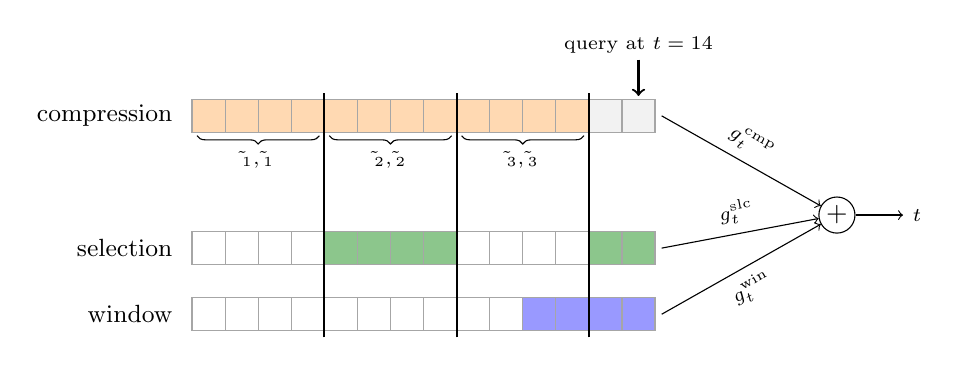
\begin{tikzpicture}[x=0.42cm,y=0.42cm]
  % compression row
  \foreach \j in {0,...,11}{\draw[gray!70,fill=orange!30] (\j,0) rectangle ++(1,1);}
  \foreach \j in {12,13}{\draw[gray!70,fill=gray!10] (\j,0) rectangle ++(1,1);}
  \foreach \bb/\nm in {0/1,1/2,2/3}{\draw[decorate,decoration={brace,amplitude=3pt,mirror}] (4*\bb+0.15,-0.1) -- (4*\bb+3.85,-0.1) node[midway,below=2pt]{\scriptsize $\tilde{\vk}_{\nm},\tilde{\vv}_{\nm}$};}
  \node[left] at (-0.3,0.5) {\small compression};
  % selection row
  \foreach \j in {0,...,13}{\draw[gray!70] (\j,-4) rectangle ++(1,1);}
  \foreach \j in {4,5,6,7,12,13}{\fill[green!50!black!45] (\j,-4) rectangle ++(1,1);}
  \foreach \j in {0,...,13}{\draw[gray!70] (\j,-4) rectangle ++(1,1);}
  \node[left] at (-0.3,-3.5) {\small selection};
  % window row
  \foreach \j in {10,...,13}{\fill[blue!40] (\j,-6) rectangle ++(1,1);}
  \foreach \j in {0,...,13}{\draw[gray!70] (\j,-6) rectangle ++(1,1);}
  \node[left] at (-0.3,-5.5) {\small window};
  % block separators
  \foreach \x in {4,8,12}{\draw[black,thick] (\x,-6.2) -- (\x,1.2);}
  % query
  \draw[->,thick] (13.5,2.2) -- (13.5,1.1);
  \node[above] at (13.5,2.1) {\scriptsize query at $t=14$};
  % gates
  \node[draw,circle,inner sep=1pt] (sum) at (19.5,-2.5) {$+$};
  \draw[->] (14.2,0.5) -- node[above,sloped]{\scriptsize $g^{\mathrm{cmp}}_t$} (sum);
  \draw[->] (14.2,-3.5) -- node[above,sloped]{\scriptsize $g^{\mathrm{slc}}_t$} (sum);
  \draw[->] (14.2,-5.5) -- node[below,sloped]{\scriptsize $g^{\mathrm{win}}_t$} (sum);
  \draw[->] (sum) -- (21.5,-2.5) node[right]{$\vo_t$};
\end{tikzpicture}
\caption{The three NSA branches for a query at $t=14$, with blocks of $B=\ell=\Delta=4$ tokens
(black separators). Compression: each of the three complete blocks becomes one compressed
token $(\tilde{\vk}_i,\tilde{\vv}_i)$; the incomplete current block (grey) is not compressed yet. Selection: the current block
and the $k-1=1$ earlier block with the highest compressed-attention importance are read at full
resolution. Window: the last $w=4$ tokens. The three outputs are mixed by sigmoid gates.}
\label{fig:c04-nsa}
\end{figure}

\subsection{Algorithms, kernel design and complexity}

\Cref{alg:c04-nsa} gives the forward pass for one GQA group; it is also the training forward
pass, since NSA is used identically in training and inference.

\begin{algorithm}[t]
\caption{NSA forward pass for one GQA group (training or prefill)}\label{alg:c04-nsa}
\begin{algorithmic}[1]
\Require queries $\vq^{(h)}_t$ for the $G$ heads of the group; shared $\vk_t,\vv_t$; gates $g^{c,(h)}_t$; $\ell,\Delta,B,k,w$
\Ensure outputs $\vo^{(h)}_t$
\State Compressed keys/values $\tilde\vk_i,\tilde\vv_i$ from \eqref{eq:c04-nsa-cmp} for all complete blocks
\For{$t=1,\dots,T$ \textbf{in parallel}}
  \For{$h=1,\dots,G$}
    \State $\vec p^{(h)}\gets$ softmax over compressed keys complete by $t$;\quad $\vo^{\mathrm{cmp},(h)}\gets\sum_i p^{(h)}_i\tilde\vv_i$
  \EndFor
  \State $p'\gets$ map $\sum_h\vec p^{(h)}$ to selection blocks by \eqref{eq:c04-nsa-map}; force the always-on blocks
  \State $\mathcal{S}_t\gets$ top-$k$ blocks of $p'$ \Comment{shared by the whole group}
  \State Load each block in $\mathcal{S}_t$ once; $\vo^{\mathrm{slc},(h)}\gets$ causal attention of $\vq^{(h)}_t$ over them, for all $h$
  \State $\vo^{\mathrm{win},(h)}\gets$ attention of $\vq^{(h)}_t$ over the last $w$ tokens
  \State $\vo^{(h)}_t\gets g^{\mathrm{cmp},(h)}_t\vo^{\mathrm{cmp},(h)}+g^{\mathrm{slc},(h)}_t\vo^{\mathrm{slc},(h)}+g^{\mathrm{win},(h)}_t\vo^{\mathrm{win},(h)}$
\EndFor
\end{algorithmic}
\end{algorithm}

\paragraph{Kernel design.}
The selection branch is the part that needs a new kernel, because each query reads a different
set of blocks. The paper's design rests on three decisions, which the \fla{} kernel follows:
\begin{itemize}
  \item \emph{Group-centric data loading.} One kernel instance handles one position $t$ and one
  key--value head, and loads the queries of all $G$ heads of the group at once, a $G\times d_k$
  tile, together with the group's shared block indices.
  \item \emph{Shared KV fetching.} The instance walks through the $k$ selected blocks, loading each
  contiguous $B\times d_k$ key block and $B\times d_v$ value block into on-chip SRAM once, and uses
  it for all $G$ queries. The product of a $G\times d_k$ tile with a $d_k\times B$ tile is a small
  matrix multiplication that tensor cores can execute; a single query would only give a
  matrix--vector product.
  \item \emph{Outer loop on the grid.} Every instance performs about the same amount of work
  ($k$ blocks), so the positions can simply be distributed over the GPU's scheduling grid with
  good load balance.
\end{itemize}

\paragraph{Cost.}
Per query, the three branches cost $\bigO(N_td_k)$ with $N_t$ from \eqref{eq:c04-nsa-count},
plus $\bigO((t/\Delta)\log k)$ for the top-$k$. Prefill therefore costs
$\bigO\big(T(T/\Delta+kB+w)d_k\big)$: still quadratic, but with constant $1/\Delta$. During
decoding the step reads $\approx t/\Delta+kB+w$ cached entries per key--value head instead of $t$,
which is the relevant saving when decoding is memory-bound. Memory is \emph{not} reduced: all
keys and values must stay cached because any block may be selected later, and the compressed
keys and values add a fraction $1/\Delta$ on top.

A decoding step appends $(\vk_t,\vv_t)$ to the cache, appends a new compressed key and value
whenever a compression block completes, and then runs the body of the loop over $t$ in
\cref{alg:c04-nsa} for the single position $t$.

\subsection{Implementation walkthrough (unofficial \fla{} code)}

\begin{implnote}[title={In the code: the attention module and its defaults}]
\code{NativeSparseAttention} in
\repofile{repos/fla-org__native-sparse-attention/native_sparse_attention/modeling_nsa.py} has the
usual \code{q_proj}, \code{k_proj}, \code{v_proj}, \code{o_proj} and one extra linear layer,
\code{g_proj}, with $3H$ outputs: \code{g_cmp, g_slc, g_swa = g.sigmoid().unbind(-1)} gives one
gate per head and branch. Rotary embeddings are applied to $\vq,\vk$ before all branches. The
defaults in \code{NSAConfig}
(\repofile{repos/fla-org__native-sparse-attention/native_sparse_attention/configuration_nsa.py})
are \code{block_size=64}, \code{block_counts=16} (the docstring of \code{naive_nsa} says 16 is
the paper's value), \code{window_size=512}, 64 query heads and 4 key--value heads. The example
\repofile{repos/fla-org__native-sparse-attention/configs/nsa_340M.json} uses 32 query heads and 2
key--value heads, a group size of 16. That is not arbitrary: \code{parallel_nsa} asserts
\code{"Group size must be a multiple of 16 in NSA"}, because the group's queries form the rows of
the tile passed to \code{tl.dot}, which needs at least 16 rows.
\end{implnote}

\begin{implnote}[title={In the code: \texttt{parallel\_nsa}, the three branches}]
\code{parallel_nsa} in
\repofile{repos/fla-org__native-sparse-attention/native_sparse_attention/ops/parallel.py} takes
\code{q} of shape \code{[B, T, HQ, K]}, \code{k}, \code{v} of shape \code{[B, T, H, K]}, three gate
tensors of shape \code{[B, T, HQ]}, \code{block_counts} and \code{window_size}:
\begin{lstlisting}[caption={Excerpt from \texttt{repos/\allowbreak{}fla-org\_\_native-sparse-attention/\allowbreak{}native\_sparse\_attention/\allowbreak{}ops/\allowbreak{}parallel.py}},label={lst:c04-nsa-parallel}]
    assert q.shape[2] % (k.shape[2] * 16) == 0, "Group size must be a multiple of 16 in NSA"

    k_cmp, v_cmp = mean_pooling(k, block_size, cu_seqlens), mean_pooling(v, block_size, cu_seqlens)
    o_cmp, lse_cmp = None, None
    if g_cmp is not None:
        o_cmp, lse_cmp = parallel_nsa_compression(
            q=q,
            k=k_cmp,
            v=v_cmp,
            # ...
        )
        # ...
        block_indices = parallel_nsa_topk(
            q=q,
            k=k_cmp,
            lse=lse_cmp,
            block_counts=block_counts,
            # ...
        )
    o_slc = ParallelNSAFunction.apply(q, k, v, block_indices, block_counts, block_size, scale, cu_seqlens)
    o = o_slc * g_slc.unsqueeze(-1)
    if o_cmp is not None:
        o = torch.addcmul(o, o_cmp, g_cmp.unsqueeze(-1))
    # ...
\end{lstlisting}
Compression is mean pooling (\code{mean_pooling} from \fla) with block length and stride both
equal to \code{block_size}. The compression branch returns its log-sum-exp \code{lse_cmp}, which
the top-$k$ kernel reuses so that the importance $p=\exp(z-\lambda)$ costs one dot product per
compressed key. The elided lines compute the window branch with the standard FlashAttention
kernel, \code{flash_attn_func(q, k, v, causal=True, window_size=(window_size-1, 0))}, i.e.\
\code{window_size} tokens including the current one, and add it with gate \code{g_swa}.
\end{implnote}

\begin{implnote}[title={In the code: the compression and top-$k$ kernels}]
\code{parallel_nsa_compression_fwd_kernel} runs one program per (position, value tile,
batch$\times$head) and processes the $G$ query heads of a group together. It visits only the
\code{NC = (i_t + 1) // BS} complete blocks (``incomplete compression blocks are not
included''), with an online softmax, and stores the output and the LSE.

\code{parallel_nsa_kernel_topk} implements the README's ``online top-$k$ selection kernel that
avoids materializing the attention matrix''. For a position $t$ and key--value head it walks over
the compressed keys in tiles of \code{BC}; for strictly earlier blocks it computes
\code{tl.exp(b_s - b_lse[:, None])}, the compressed attention probability, assigns
\code{float(1.0)} to the current block (\code{i_t // BS == o_c}) so that it is always kept, and
sums over the $G$ heads with \code{tl.sum(b_p, 0)}: exactly the group importance $p'_t$. A
running list of the best candidates is maintained with bitonic merges (\code{_bitonic_merge} in
\repofile{repos/fla-org__native-sparse-attention/native_sparse_attention/ops/utils.py}, an
argsort built from compare-and-swap steps that suits SIMD hardware). The number of kept indices
is rounded up to a power of two; unused slots hold $-1$. Because this kernel only outputs
integers, no gradient flows through it.
\end{implnote}

\begin{implnote}[title={In the code: the selection kernel}]
\code{parallel_nsa_fwd_kernel} is launched on the grid \code{(T, NV, B * H)}: one program per
position, value tile and (batch, key--value head). It loads the group's queries as
\code{b_q} of shape \code{[G, BK]} and then loops over the selected blocks:
\begin{lstlisting}[caption={Excerpt from \texttt{repos/\allowbreak{}fla-org\_\_native-sparse-attention/\allowbreak{}native\_sparse\_attention/\allowbreak{}ops/\allowbreak{}parallel.py}},label={lst:c04-nsa-kernel}]
    b_m = tl.full([G], float('-inf'), dtype=tl.float32)
    b_acc = tl.zeros([G], dtype=tl.float32)
    for i in range(NS):
        i_s = tl.load(block_indices + i).to(tl.int32) * BS
        if i_s <= i_t and i_s >= 0:
            p_k = tl.make_block_ptr(k, (K, T), (1, H*K), (0, i_s), (BK, BS), (0, 1))
            p_v = tl.make_block_ptr(v, (T, V), (H*V, 1), (i_s, i_v * BV), (BS, BV), (1, 0))
            # [BK, BS]
            b_k = tl.load(p_k, boundary_check=(0, 1))
            # [BS, BV]
            b_v = tl.load(p_v, boundary_check=(0, 1))
            # [G, BS]
            b_s = tl.dot(b_q, b_k)
            b_s = tl.where((i_t >= (i_s + tl.arange(0, BS)))[None, :], b_s, float('-inf'))

            # [G]
            b_m, b_mp = tl.maximum(b_m, tl.max(b_s, 1)), b_m
            b_r = tl.exp(b_mp - b_m)
            # [G, BS]
            b_p = tl.exp(b_s - b_m[:, None])
            # [G]
            b_acc = b_acc * b_r + tl.sum(b_p, 1)
            # [G, BV]
            b_o = b_o * b_r[:, None] + tl.dot(b_p.to(b_q.dtype), b_v)

            b_mp = b_m
    b_o = b_o / b_acc[:, None]
    b_m += tl.log(b_acc)
\end{lstlisting}
Each iteration fetches one contiguous key block and one value block through block pointers
(shared KV fetching), multiplies the $G\times$\code{BK} query tile by it (\code{tl.dot}, the
group-centric product), applies the causal mask inside the block, and updates the running
maximum \code{b_m}, normalizer \code{b_acc} and output \code{b_o}: the online softmax, i.e.\
\cref{prop:c04-merge} applied one block at a time. The final LSE is stored for the backward pass.

The backward pass (\code{parallel_nsa_bwd}) has a query-side kernel (each position revisits its
blocks) and a key-side kernel. The key side needs the inverse map, ``which positions selected
this block?'', which \code{parallel_nsa_kernel_mask} builds as a dense boolean tensor
\code{[B, T, H, NS]}. A preprocessing kernel computes $\bar\vo\T\vo$ per position, the
correction term of \eqref{eq:c04-merge-bwd}.
\end{implnote}

\begin{implnote}[title={In the code: reference version, tests, and differences from the paper}]
\repofile{repos/fla-org__native-sparse-attention/native_sparse_attention/ops/naive.py} contains
loop-based references: \code{naive_nsa} (selection and window branches, one query at a time) and
\code{naive_nsa_compression} (compression and top-$k$; its mask \code{(t - BS + 1) // BS < c}
hides incomplete blocks, and \code{local_mask} forces the current block). The tests
\repofile{repos/fla-org__native-sparse-attention/tests/test_nsa.py} and
\repofile{repos/fla-org__native-sparse-attention/tests/test_nsa_with_compression.py} compare the
Triton kernels with these references. Compared with the paper, this implementation
(i) compresses by mean pooling rather than a learned MLP $\varphi$, (ii) uses $\ell=\Delta=B$,
so \eqref{eq:c04-nsa-map} is the identity, (iii) shares keys and values across the three branches,
(iv) forces only the current block, and (v) requires GQA groups whose size is a multiple of 16.
\end{implnote}

\subsection{From-scratch reference implementation}

\Cref{lst:c04-nsa-ref} implements \eqref{eq:c04-nsa-combine}--\eqref{eq:c04-nsa-slc} for one GQA
group with dense masks and the \fla{} simplifications ($\ell=\Delta=B$, mean pooling, shared
$\vk,\vv$, current block forced).

\begin{lstlisting}[caption={Reference implementation (ours): the three NSA branches for one GQA group.},label={lst:c04-nsa-ref}]
def nsa_group(q, k, v, g, B, n_sel, w):
    # q: [G, T, d] queries of one GQA group; k, v: [T, d] shared; g: [G, T, 3] gates
    G, T, d = q.shape
    nb = T // B                                            # assume B divides T
    kc, vc = k.view(nb, B, d).mean(1), v.view(nb, B, d).mean(1)   # compression
    t, c = torch.arange(T)[:, None], torch.arange(nb)[None, :]
    done = (c + 1) * B - 1 <= t                            # complete blocks only
    sc = (q @ kc.T) / d**0.5                               # [G, T, nb]
    p = sc.masked_fill(~done, float('-inf')).softmax(-1).nan_to_num()
    o_cmp = p @ vc
    imp = p.sum(0)                                         # importance shared by the group
    imp = imp.masked_fill(c == t // B, float('inf'))       # current block always kept
    imp = imp.masked_fill(c > t // B, float('-inf'))       # future blocks never
    idx = imp.topk(min(n_sel, nb), dim=-1).indices
    sel = torch.zeros(T, nb, dtype=torch.bool).scatter_(1, idx, True) & (c <= t // B)
    causal = torch.ones(T, T, dtype=torch.bool).tril()
    s = (q @ k.T) / d**0.5                                 # [G, T, T]
    m_slc = sel[:, torch.arange(T) // B] & causal          # expand blocks to tokens
    o_slc = s.masked_fill(~m_slc, float('-inf')).softmax(-1) @ v
    m_win = causal & (t - torch.arange(T)[None, :] < w)    # last w tokens incl. current
    o_win = s.masked_fill(~m_win, float('-inf')).softmax(-1) @ v
    return g[..., 0:1] * o_cmp + g[..., 1:2] * o_slc + g[..., 2:3] * o_win
\end{lstlisting}

A NumPy transcription ($G=4$, $T=64$, $d=8$, $B=8$) confirms \cref{prop:c04-nsa-special}
(difference $0$), causality of the full gated output and of the selection, that every query keeps
its current block and at most $k$ blocks, and \cref{prop:c04-nsa-overlap} for four $(\ell,\Delta,B)$
settings.

\begin{results}
\emph{From \repofile{repos/fla-org__native-sparse-attention/README.md} (unofficial
implementation):} a benchmark table of execution times for the \fla{} kernels against
FlashAttention. The README does not state the configuration. The benchmark script
\repofile{repos/fla-org__native-sparse-attention/benchmarks/benchmark_nsa.py} (whose current
version may differ from the one that produced the table) labels the y-axis in milliseconds and
uses 64 query heads, 4 key--value heads, head dimension 128, 16 selected blocks of 64 tokens, a
64-token window and random block indices, i.e.\ no compression branch. Selected rows (``bwd''
columns time forward plus backward):
\begin{center}
\small
\begin{tabular}{rrrrr}
\toprule
$T$ & NSA fwd & NSA bwd & Flash fwd & Flash bwd\\
\midrule
1024 & 1.04 & 5.09 & 0.30 & 1.32\\
4096 & 4.87 & 23.08 & 3.52 & 14.19\\
8192 & 9.95 & 49.58 & 13.46 & 52.57\\
16384 & 20.16 & 116.30 & 53.63 & 204.35\\
\bottomrule
\end{tabular}
\end{center}
The sparse kernel is slower than dense FlashAttention at short lengths and faster from 8K tokens
on, because its cost grows linearly in $T$ for a fixed budget while dense attention grows
quadratically.

\emph{Paper (no numbers in this repository):} the abstract reports that models pretrained with NSA
match or exceed full-attention models on general benchmarks, long-context tasks and
instruction-based reasoning, while being substantially faster than full attention on long
sequences in decoding, forward and backward passes. See the paper for numbers.
\end{results}

\subsection{Discussion}

\textbf{Strengths.} NSA gives every query three complementary views: a complete but blurred view
of the whole past (compression), a sharp view of the few regions that matter (selection) and a
sharp view of the recent past (window). The selector is trained through the compression branch,
the gates let the model weight the views per head and token, and the whole design is built
around what GPUs do well: contiguous block loads and small matrix products shared by a GQA group.

\textbf{Limitations.} The design couples the algorithm to GQA (selection is shared by a group, and
the \fla{} kernel needs groups of at least 16 heads) and needs custom kernels for forward and
backward. The compression branch still reads $t/\Delta$ entries per query, so cost is quadratic
in the long run. As with MoBA, the KV cache is not reduced: NSA is access control, not retention
control. Block-level selection can still miss isolated tokens, although the compression and window
branches soften this.

\textbf{Relations.} MoBA (\cref{sec:c04-moba}) is the parameter-free cousin: mean-pooled keys
instead of learned compressed attention, one softmax instead of three gated branches, unmodified
FlashAttention instead of a new kernel. RATTENTION (next section) also pairs a window with a
global summary, but its summary is a fixed-size linear-attention state rather than a growing list
of compressed tokens. Combining attention with recurrent summaries in separate layers is the
subject of \cref{ch:hybrid}.

% =====================================================================================
\section{RATTENTION: a minimal window plus residual linear attention}\label{sec:c04-rattention}

\subsection{Motivation}

\emph{Local--global} models interleave sliding-window layers with full-attention layers: the
local layers are cheap and keep a bounded cache, the global layers provide long-range recall.
The open question is the window size $w$. The RATTENTION README points out that frontier models
choose conservative windows; both Mistral \citep{c04-jiang2023mistral} and Gemma~2
\citep{c04-gemma2024gemma2} use a 4096-token window within an 8192-token pretraining context.
With such a window, a local layer behaves exactly like a global one on any sequence of up to 4K
tokens, so the efficiency benefit appears only on long inputs. Shrinking the window helps
efficiency, but naively it hurts quality, because tokens outside the window become invisible to
the local layers.

RATTENTION \citep{wang2025rattention} (Apple) removes the cliff at the window edge. Next to
the window it adds a \emph{residual linear attention} (RLA) branch whose state accumulates exactly
the tokens that have left the window. Recent tokens are read exactly by softmax attention; older
tokens are read approximately through a fixed-size linear-attention memory (\cref{ch:linear}).
With this safety net, the README reports that a 512-token window can replace a 4K window. The RLA
branch reuses the attention layer's own query, key and value projections and adds no weights
beyond two normalization scales.

\begin{taxonomy}
\textbf{Representation:} implicit (a windowed KV cache plus a recurrent state, both by-products
of the forward pass).
\textbf{Update dynamics:} online (each step evicts one token from the window and writes it into
the state).
\textbf{Persistence:} short-term; Table I of \citet{zhoubian2026memory} lists RATTENTION as
online, short-term, ``local--global minimal sliding window''.
\textbf{Update rule:} survey Table II places RATTENTION under ``admission, eviction, and
consolidation'': tokens are evicted from the exact store and consolidated into a compressed state.
The survey's Section III-B uses it as the example of local--global structure and memory retention.
\end{taxonomy}

\subsection{Formulation}

Fix a head of a local layer. Following the code, the window contains the current token and the
$w$ tokens before it, as in \eqref{eq:c04-swa}.

\paragraph{Window branch.} Ordinary softmax attention with rotary position embeddings (RoPE,
\cref{ch:foundations}); write $\hat\vq_t,\hat\vk_s$ for the rotated vectors:
\begin{equation}\label{eq:c04-ratt-swa}
  \vo^{\mathrm{swa}}_t=\sum_{s=\max(1,t-w)}^{t}
  \frac{\exp(\hat\vq_t\T\hat\vk_s/\sqrt{d_k})}{\sum_{s'=\max(1,t-w)}^{t}\exp(\hat\vq_t\T\hat\vk_{s'}/\sqrt{d_k})}\,\vv_s .
\end{equation}

\paragraph{Residual linear attention branch.} Linear attention over \emph{exactly} the tokens that
are no longer in the window, using the unrotated, unscaled $\vq_t,\vk_s$ and a positive feature
map:
\begin{equation}\label{eq:c04-ratt-rla}
  \vo^{\mathrm{rla}}_t=\sum_{s=1}^{t-w-1}\big(\phi(\vq_t)\T\phi(\vk_s)\big)\vv_s=\mS_t\,\phi(\vq_t),
  \qquad \mS_t=\sum_{s=1}^{t-w-1}\vv_s\phi(\vk_s)\T\in\R^{d_v\times 2d_k},
\end{equation}
with the default feature map
\begin{equation}\label{eq:c04-ratt-phi}
  \phi(\vx)=\big[\softmax(\vx);\;\softmax(-\vx)\big]\in\R^{2d_k},
\end{equation}
the concatenation of a softmax over the coordinates of $\vx$ and one over the coordinates of
$-\vx$ (the code cites the Hedgehog feature maps of \citet{c04-zhang2024hedgehog}; a ReLU
variant $[\ReLU(\vx);\ReLU(-\vx)]$ is also implemented). This is the plainest possible linear
attention: no decay, no gate, no delta rule, no denominator. The state starts at zero, or at a
learned $\mS_0=\sum_{j}\vv^{\mathrm{meta}}_j\phi(\vk^{\mathrm{meta}}_j)\T$ built from learned
``meta tokens'' if that option is enabled.

\paragraph{Combination.} Each branch is normalized per head by an RMSNorm with its own learned
scale, and the two are added:
\begin{equation}\label{eq:c04-ratt-mix}
  \vy_t=\vec\gamma^{\mathrm{swa}}\had\frac{\vo^{\mathrm{swa}}_t}{\mathrm{rms}(\vo^{\mathrm{swa}}_t)}
  +\vec\gamma^{\mathrm{rla}}\had\frac{\vo^{\mathrm{rla}}_t}{\mathrm{rms}(\vo^{\mathrm{rla}}_t)},
  \qquad \mathrm{rms}(\vx)=\sqrt{\tfrac{1}{d_v}\textstyle\sum_i x_i^2+\epsilon},
\end{equation}
after which the heads are concatenated and projected by $\mW_O$ as usual.

Why normalize? The window output is a convex combination of at most $w+1$ values, so its size is
bounded by the largest value. The RLA output is an \emph{unnormalized} sum: the features are
positive and each weight $\phi(\vq)\T\phi(\vk)$ lies in $(0,2]$ (two inner products of probability
vectors), so $\vo^{\mathrm{rla}}_t$ grows roughly in proportion to the number of evicted tokens.
Normalizing each branch to unit RMS puts both on the same scale, removes the need for the
usual linear-attention denominator $\sum_s\phi(\vq_t)\T\phi(\vk_s)$, and leaves the relative weight
of the two memories to the learned scales $\vec\gamma$.

\begin{proposition}[Exact partition of the context]\label{prop:c04-ratt-partition}
For every $t$, the index sets of the two branches,
$\mathcal{I}^{\mathrm{swa}}_t=\{\max(1,t-w),\dots,t\}$ and $\mathcal{I}^{\mathrm{rla}}_t=\{1,\dots,t-w-1\}$,
are disjoint and their union is $\{1,\dots,t\}$. Hence every past token is read by exactly one
branch: exactly if it is among the $w+1$ most recent, through the linear state otherwise.
\end{proposition}
\begin{proof}
If $t\le w+1$, $\mathcal{I}^{\mathrm{rla}}_t$ is empty and $\mathcal{I}^{\mathrm{swa}}_t=\{1,\dots,t\}$.
Otherwise the first set is $\{t-w,\dots,t\}$ and the second $\{1,\dots,t-w-1\}$; they are
consecutive integer ranges that meet at $t-w-1<t-w$.
\end{proof}

\paragraph{Recurrent view: a delayed write.}
From \eqref{eq:c04-ratt-rla}, $\mS_t-\mS_{t-1}$ contains exactly one term, the token that has just
left the window:
\begin{equation}\label{eq:c04-ratt-recur}
  \mS_t=\mS_{t-1}+\vv_{t-w-1}\,\phi(\vk_{t-w-1})\T \quad(t\ge w+2),\qquad \vo^{\mathrm{rla}}_t=\mS_t\,\phi(\vq_t).
\end{equation}
This is the plain linear-attention write $\mS_t=\mS_{t-1}+\vv_t\vk_t\T$ of \cref{ch:linear},
delayed by $w+1$ steps. Define shifted inputs $\vk'_t=\vk_{t-w-1}$, $\vv'_t=\vv_{t-w-1}$, with
$\vv'_t=\mathbf{0}$ (and $\vk'_t$ arbitrary) for $t\le w+1$. Substituting $s=s'+w+1$ in
\eqref{eq:c04-ratt-rla} gives
\begin{equation}\label{eq:c04-ratt-shift}
  \vo^{\mathrm{rla}}_t=\sum_{s'=1}^{t}\big(\phi(\vq_t)\T\phi(\vk'_{s'})\big)\vv'_{s'} ,
\end{equation}
which is \emph{ordinary causal linear attention} on $(\phi(\vq_t),\phi(\vk'_t),\vv'_t)$. Any
linear-attention kernel can therefore compute the RLA branch unchanged, after shifting its inputs.
A detail that matters for the code: the zero padding may be applied to the raw keys before the
feature map, although $\phi(\mathbf 0)=\tfrac{1}{d_k}\mathbf 1\ne\mathbf 0$ for the softmax map,
because every padded position also has $\vv'=\mathbf 0$ and so contributes
$\phi(\mathbf 0)\T\phi(\vq)\cdot\mathbf 0=\mathbf 0$.

\paragraph{Chunkwise view.}
With chunks of size $C$ and $\mQ_{[i]},\mK'_{[i]},\mV'_{[i]}$ the rows of chunk $i$ (features
applied row-wise), the chunkwise form of \cref{ch:linear} reads
\begin{equation}\label{eq:c04-ratt-chunk}
  \mO^{\mathrm{rla}}_{[i]}=\phi(\mQ_{[i]})\,\mS_{[i-1]}\T+\Big(\big(\phi(\mQ_{[i]})\phi(\mK'_{[i]})\T\big)\had\mM_C\Big)\mV'_{[i]},\qquad
  \mS_{[i]}=\mS_{[i-1]}+\mV'^{\top}_{[i]}\phi(\mK'_{[i]}),
\end{equation}
where $\mM_C$ is the $C\times C$ lower-triangular matrix of ones and $\mS_{[i]}$ is the state after
chunk $i$. The first term reads the state accumulated before the chunk (inter-chunk), the second
handles pairs inside the chunk (intra-chunk); their sum is \eqref{eq:c04-ratt-shift}.

\begin{figure}[t]
\centering
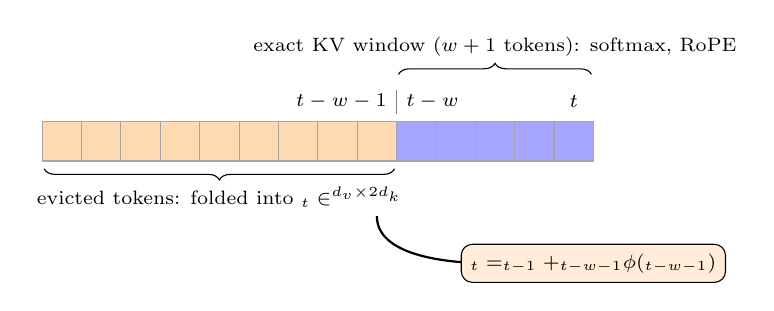
\begin{tikzpicture}[x=0.5cm,y=0.5cm]
  \foreach \j in {1,...,9}{\draw[gray!70,fill=orange!30] (\j,0) rectangle ++(1,1);}
  \foreach \j in {10,...,14}{\draw[gray!70,fill=blue!35] (\j,0) rectangle ++(1,1);}
  \node at (14.5,1.5) {\scriptsize $t$};
  \node[anchor=west] at (10.0,1.5) {\scriptsize $t-w$};
  \node[anchor=east] at (10.0,1.5) {\scriptsize $t-w-1$};
  \draw[gray] (10.0,1.2) -- (10.0,1.8);
  \draw[decorate,decoration={brace,amplitude=4pt}] (10.05,2.2) -- (14.95,2.2) node[midway,above=3pt]{\scriptsize exact KV window ($w+1$ tokens): softmax, RoPE};
  \draw[decorate,decoration={brace,amplitude=4pt,mirror}] (1.05,-0.2) -- (9.95,-0.2) node[midway,below=3pt]{\scriptsize evicted tokens: folded into $\mS_t\in\R^{d_v\times 2d_k}$};
  \draw[->,thick] (9.5,-1.4) .. controls (9.5,-2.6) and (12,-2.6) .. (12.5,-2.6);
  \node[draw,rounded corners,fill=orange!15] at (15.0,-2.6) {\scriptsize $\mS_t=\mS_{t-1}+\vv_{t-w-1}\phi(\vk_{t-w-1})\T$};
\end{tikzpicture}
\caption{RATTENTION's partition of the context at time $t$ (\cref{prop:c04-ratt-partition}). The
$w+1$ most recent tokens (blue) are kept exactly and read by sliding-window softmax attention; each
token that leaves the window (orange) is written once into a fixed-size linear-attention state.}
\label{fig:c04-ratt}
\end{figure}

\subsection{The minimal-window question}

What does a smaller window buy? Consider a model in which a fraction $\rho$ of the attention layers
are local and the rest global. At context length $T$ the global layers cache $T$ tokens and the
local layers $\min(w+1,T)$, so the KV memory relative to an all-global model is
$(1-\rho)+\rho\min(w+1,T)/T$, a saving of
\begin{equation}\label{eq:c04-ratt-saving}
  \text{saving}(T)=\rho\Big(1-\frac{\min(w+1,T)}{T}\Big)
\end{equation}
(plus a constant $2d_kd_v$ per head for the RLA state). With a 4K window there is no saving for
$T\le4\mathrm{K}$, as the README notes. With a 1K window, $\rho=3/4$ and $T=4\mathrm{K}$, the saving
is $\tfrac34\cdot\tfrac34\approx56\%$, which matches the README's ``$\sim$56\% KV cache savings''
for a 12B local--global model at sequences up to 4K tokens. The README does not state the layer
ratio; $\rho=3/4$ is our reconstruction of how the figure arises.

Compute behaves similarly: per token and head the window costs about $(w+1)(d_k+d_v)$
multiply--adds, while the RLA state read and write cost about $4d_kd_v$, with $d_k=d_v=128$ about
as much as a window of a few hundred tokens. A 512-token window plus RLA should therefore train no
slower than a 4K window, given an efficient kernel; the README claims exactly this. The quality
side of the trade-off is empirical (see the results box).

\subsection{Algorithms and complexity}

\begin{algorithm}[t]
\caption{RATTENTION local layer, training or prefill (one head)}\label{alg:c04-ratt-prefill}
\begin{algorithmic}[1]
\Require $\mQ,\mK\in\R^{T\times d_k}$, $\mV\in\R^{T\times d_v}$, window $w$, chunk size $C$, state $\mS_0$
\State $\mO^{\mathrm{swa}}\gets$ sliding-window softmax attention with RoPE \eqref{eq:c04-ratt-swa} \Comment{FlashAttention with a window mask}
\State $\mK'\gets$ shift $\mK$ down by $w+1$ rows, zero padded;\quad $\mV'\gets$ same for $\mV$
\State $\mS\gets\mS_0$
\For{each chunk $i$}
  \State $\mO^{\mathrm{rla}}_{[i]}\gets\phi(\mQ_{[i]})\mS\T+\big((\phi(\mQ_{[i]})\phi(\mK'_{[i]})\T)\had\mM_C\big)\mV'_{[i]}$
  \State $\mS\gets\mS+\mV'^{\top}_{[i]}\phi(\mK'_{[i]})$
\EndFor
\State \Return $\vec\gamma^{\mathrm{swa}}\had\mathrm{RMSNorm}(\mO^{\mathrm{swa}})+\vec\gamma^{\mathrm{rla}}\had\mathrm{RMSNorm}(\mO^{\mathrm{rla}})$ \Comment{row-wise}
\end{algorithmic}
\end{algorithm}

\begin{algorithm}[t]
\caption{RATTENTION decoding step at time $t$ (one head)}\label{alg:c04-ratt-decode}
\begin{algorithmic}[1]
\Require ring buffer $\mathcal{W}$ of the last $w+1$ pairs $(\vk_s,\vv_s)$; state $\mS$
\State Push $(\vk_t,\vv_t)$ into $\mathcal{W}$
\If{$\abs{\mathcal{W}}>w+1$}
  \State Pop the oldest pair $(\vk_{t-w-1},\vv_{t-w-1})$;\quad $\mS\gets\mS+\vv_{t-w-1}\phi(\vk_{t-w-1})\T$ \Comment{evict and consolidate}
\EndIf
\State $\vo^{\mathrm{swa}}\gets$ softmax attention of $\hat\vq_t$ over $\mathcal{W}$;\quad $\vo^{\mathrm{rla}}\gets\mS\phi(\vq_t)$
\State \Return $\vec\gamma^{\mathrm{swa}}\had\mathrm{RMSNorm}(\vo^{\mathrm{swa}})+\vec\gamma^{\mathrm{rla}}\had\mathrm{RMSNorm}(\vo^{\mathrm{rla}})$
\end{algorithmic}
\end{algorithm}

Prefill costs $\bigO(Twd_k)$ for the window and $\bigO(TCd_k+Td_kd_v)$ for the chunkwise RLA:
linear in $T$. A decoding step costs $\bigO(wd_k+d_kd_v)$ and the memory of a local layer is
$(w+1)(d_k+d_v)+2d_kd_v$ numbers per head, \emph{independent of} $t$. Global layers keep their
full cache.

\subsection{Implementation walkthrough}

The code lives in AXLearn, Apple's JAX library; the mirror contains only the folder
\repofile{repos/apple__axlearn/axlearn/common/rattention}. Kernels are written in Pallas, JAX's
kernel language, and target TPUs.

\begin{implnote}[title={In the code: the \texttt{RAttention} layer}]
\code{RAttention} in \repofile{repos/apple__axlearn/axlearn/common/rattention/rattention.py}
subclasses AXLearn's \code{FlashAttention} layer. Its config adds \code{sliding_window_size}
(default 1024), \code{residual_la} (the RLA config; \code{None} disables the branch),
\code{rope_theta} (default 500000) and \code{mixing_norm} (default: \code{GroupRMSNorm} from
\repofile{repos/apple__axlearn/axlearn/common/rattention/utils.py}, an RMSNorm per head with a
learned scale of shape \code{[num_heads, head_dim]}). The window mask is AXLearn's
\code{SlidingWindowAttentionBias}; according to AXLearn's \code{attention_bias.py} (outside the
mirrored folder), window size $w$ means attending to the token itself and $w$ tokens to the left,
the convention of \eqref{eq:c04-swa}. Because the RLA branch must see \emph{unrotated} queries and
keys, RAttention refuses a \code{RoFormerQKVLinear} input projection and applies RoPE itself, only
on the window branch. The final assembly in \code{_forward_for_mode} is
\eqref{eq:c04-ratt-mix}:
\begin{lstlisting}[caption={Excerpt from \texttt{repos/\allowbreak{}apple\_\_axlearn/\allowbreak{}axlearn/\allowbreak{}common/\allowbreak{}rattention/\allowbreak{}rattention.py}},label={lst:c04-ratt-mix}]
        # Assemble the final results.
        if cfg.sliding_window_size >= 0:
            # ... (scale the RoPE-rotated q and k with self._scale_qk)
            swa_context, _ = self._compute_attention(
                mode=mode,
                q_proj=scaled_q_proj_rope,
                kv_state=KVState(scaled_full_k_proj_rope, full_v_proj, key_positions),
                attention_logit_biases=attention_logit_biases,
            )
            if cfg.residual_la is not None:
                swa_context = self.swa_norm(swa_context)
                # pylint: disable-next=possibly-used-before-assignment
                rla_context = self.rla_norm(rla_output)
                context = swa_context + rla_context
            else:
                context = swa_context
        else:
            context = self.rla_norm(rla_output)

        o_proj = self.o_proj(context)
\end{lstlisting}
With \code{sliding_window_size = -1} the layer degenerates to RLA only.
\end{implnote}

\begin{implnote}[title={In the code: \texttt{ResidualLinearAttention} and decoding}]
\code{ResidualLinearAttention} (same file) is configured by \code{feat_fn} (default
\code{FeatureMap("softmax")}, i.e.\ \eqref{eq:c04-ratt-phi}), \code{chunk_size} (default 512),
and two optional extras, \code{use_learned_init} (128 meta tokens per head give $\mS_0$) and
\code{use_qk_scale}; otherwise it has no parameters. The state is stored as $\mS\T$, shape
\code{[batch, heads, 2 * head_dim, head_dim]}. \code{_get_linear_attention_impl} picks the Pallas
kernel for TPU training and a \code{jax.lax.scan} reference elsewhere. Decoding uses
\code{_compute_linear_attention_step}:
\begin{lstlisting}[caption={Excerpt from \texttt{repos/\allowbreak{}apple\_\_axlearn/\allowbreak{}axlearn/\allowbreak{}common/\allowbreak{}rattention/\allowbreak{}rattention.py}},label={lst:c04-ratt-step}]
        shift_size = cfg.sliding_window_size + 1
        if cfg.sliding_window_size > 0:
            k_proj = right_shift_and_zero_pad(k_proj, shift_size)
            v_proj = right_shift_and_zero_pad(v_proj, shift_size)

        k_proj = self._repeat_kv_heads(k_proj)
        v_proj = self._repeat_kv_heads(v_proj)

        q_proj_t = q_proj.squeeze(axis=1)
        k_proj_t = jnp.take_along_axis(
            k_proj, time_step[:, None, None, None], axis=1, mode="clip"
        ).squeeze(axis=1)
        v_proj_t = jnp.take_along_axis(
            v_proj, time_step[:, None, None, None], axis=1, mode="clip"
        ).squeeze(axis=1)

        new_state = state.astype(jnp.float32) + jnp.einsum("bnk,bnv -> bnkv", k_proj_t, v_proj_t)
        output = jnp.einsum("bnk,bnkv -> bnv", q_proj_t, new_state)
        output = output[:, None, :, :]  # add seq_len dimension
        return new_state.astype(orig_dtype), output.astype(orig_dtype)
\end{lstlisting}
This is \eqref{eq:c04-ratt-recur}: after shifting by $w+1$, entry \code{time_step} of the shifted
keys is the token that just left the window; it is added to the state, and the state is read with
the current query. Note that the decoding path receives the \emph{full} key and value cache and
indexes into it; a \code{TODO} in \code{_forward_for_mode} says this should be replaced by a cache
that stores only in-window tokens, which is what \cref{alg:c04-ratt-decode} does.
\end{implnote}

\begin{implnote}[title={In the code: the Pallas kernels}]
\repofile{repos/apple__axlearn/axlearn/common/rattention/kernels/linear_attention_kernels.py}
implements \eqref{eq:c04-ratt-shift}--\eqref{eq:c04-ratt-chunk}. The entry point
\code{residual_linear_attention} shifts the raw inputs and calls a linear-attention function with a
custom VJP:
\begin{lstlisting}[caption={Excerpt from \texttt{repos/\allowbreak{}apple\_\_axlearn/\allowbreak{}axlearn/\allowbreak{}common/\allowbreak{}rattention/\allowbreak{}kernels/\allowbreak{}linear\_attention\_kernels.py}},label={lst:c04-ratt-shiftcode}]
    # Using softmax feature map, we can shift k/v as the input, which is equivalent to
    # to shift the feature map of k/v.
    k = right_shift_and_zero_pad(k, window_size + 1, axis=2)
    v = right_shift_and_zero_pad(v, window_size + 1, axis=2)
\end{lstlisting}
The comment is the $\phi(\mathbf 0)\cdot\mathbf 0=\mathbf 0$ argument above. The forward kernel
runs on the grid \code{(batch, heads, chunks)} with dimension semantics
\code{("parallel", "parallel", "arbitrary")}: chunks are processed sequentially and carry the state
from one to the next. Inside a chunk it loops over sub-chunks of 128 tokens:
\begin{lstlisting}[caption={Excerpt from \texttt{repos/\allowbreak{}apple\_\_axlearn/\allowbreak{}axlearn/\allowbreak{}common/\allowbreak{}rattention/\allowbreak{}kernels/\allowbreak{}linear\_attention\_kernels.py}},label={lst:c04-ratt-kernel}]
    def _la_forward_chunk_loop_body(t: int, h_carry_ref: Tensor):
        subchunk_idx = t
        h_block = h_carry_ref[:, :]

        q_block = q_ref[subchunk_idx, :].astype(jnp.float32)
        k_block = k_ref[subchunk_idx, :].astype(jnp.float32)
        v_block = v_ref[subchunk_idx, :].astype(jnp.float32)

        q_block_ = feat_fn.fwd(q_block)
        k_block_ = feat_fn.fwd(k_block)

        o_block_inter = _matmul_fp32(q_block_, h_block)
        intra_att = _matmul_fp32(q_block_, k_block_.T)
        o_block_intra = _matmul_fp32((intra_att * casual_mask), v_block)
        o_block = o_block_inter + o_block_intra

        next_h_block = h_block + _matmul_fp32(k_block_.T, v_block)  # [d_k, d_v]
        mutable_o_ref[subchunk_idx, :] = o_block.astype(mutable_o_ref.dtype)

        h_carry_ref[:, :] = next_h_block
\end{lstlisting}
\code{o_block_inter} and \code{o_block_intra} are the two terms of \eqref{eq:c04-ratt-chunk} and
\code{next_h_block} is the state update, all in float32 with the feature map fused into the kernel.
The README attributes the kernels' efficiency to fused operations and ``flexible state saving''
(an interleaved pattern detailed in the paper). One visible form in the code: the forward kernel
saves the state only once per \emph{chunk} (\code{mutable_ch_ref}, default chunk 512), not per 128-token
sub-chunk, and the backward kernel recomputes the sub-chunk states from it. The backward kernel
walks the chunks in reverse order (\code{chunk_dim - 1 - m} in its index maps) so that the
gradient with respect to the state can flow from later to earlier chunks. The kernels assert a head
dimension of 128 (\code{singleton_dim}), so the feature dimension is 256. The feature maps and
their hand-written derivatives (\code{sm2_fwd}, \code{sm2_bwd}, \code{relu2_fwd},
\code{relu2_bwd}) are in \repofile{repos/apple__axlearn/axlearn/common/rattention/kernels/utils.py}.
The tests compare the Pallas kernel with the \code{lax.scan} version (TPU only), decoding with the
parallel pass, and RAttention without RLA with windowed \code{FlashAttention}.
\end{implnote}

\subsection{From-scratch reference implementation}

\begin{lstlisting}[caption={Reference implementation (ours): RATTENTION for one head, parallel form and decoding step.},label={lst:c04-ratt-ref}]
def phi(x):                                        # [softmax(x), softmax(-x)]
    return torch.cat([x.softmax(-1), (-x).softmax(-1)], dim=-1)

def rms_norm(x, gamma, eps=1e-8):
    return gamma * x * torch.rsqrt((x * x).mean(-1, keepdim=True) + eps)

def rattention_head(q, k, v, q_rope, k_rope, w, g_swa, g_rla):
    # q, k: [T, d_k] unrotated; q_rope, k_rope: rotated; v: [T, d_v]
    T, d = q.shape
    i = torch.arange(T)
    lag = i[:, None] - i[None, :]
    in_win = (lag >= 0) & (lag <= w)               # current token + w to the left
    s = (q_rope @ k_rope.T) / d**0.5
    o_swa = s.masked_fill(~in_win, float('-inf')).softmax(-1) @ v
    A = (phi(q) @ phi(k).T) * (lag >= w + 1)       # evicted tokens only, no normaliser
    o_rla = A @ v
    return rms_norm(o_swa, g_swa) + rms_norm(o_rla, g_rla)

def rla_decode_step(S, q_t, k_evicted, v_evicted):
    # S: [d_v, 2*d_k]; (k_evicted, v_evicted) = token t-w-1, or zeros if t <= w+1
    S = S + torch.outer(v_evicted, phi(k_evicted))
    return S, S @ phi(q_t)
\end{lstlisting}

Our NumPy checks ($T=50$, $d_k=d_v=6$, $w=7$) confirm that the delayed-write recurrence
\eqref{eq:c04-ratt-recur}, the direct sum \eqref{eq:c04-ratt-rla} and the chunkwise form
\eqref{eq:c04-ratt-chunk} ($C\in\{4,8,16\}$) agree to $2\times10^{-15}$; that shifting raw keys
before $\phi$ is harmless; \cref{prop:c04-ratt-partition}; and that ring-buffer decoding reproduces
the parallel output of \cref{lst:c04-ratt-ref}.

\begin{results}
\emph{From \repofile{repos/apple__axlearn/axlearn/common/rattention/README.md}:}
\begin{itemize}
  \item A standard sliding-window attention with a 4K window can be replaced by RATTENTION with a
  512-token window ``without compromising performance or training speed'', with better
  long-context understanding.
  \item Mistral and Gemma~2 use a 4096-token window within an 8192-token pretraining context; a
  12B local--global model with a 4K window saves no KV cache at sequences of 4K tokens or less,
  while a 1K window saves about 56\%.
  \item A figure (no numbers in the text) compares MMLU 5-shot scores across window sizes at 3B
  scale with pretraining context 4096: naive window shrinking hurts, RATTENTION does not.
  \item The kernels' fused operations and flexible state saving make training RATTENTION with a
  512 window as efficient as SWA with a 4K window; the linear attention is parameter-free.
\end{itemize}
See the paper for the full experiments and numbers.
\end{results}

\subsection{Discussion}

\textbf{Strengths.} RATTENTION is a small, local change: one extra branch inside the local
attention layer, no new projections, and a clear division of labour fixed by
\cref{prop:c04-ratt-partition}. It turns the hard cutoff of a sliding window into a graded memory
(exact recent past, compressed distant past) and makes much smaller windows usable, which shrinks
both the KV cache and the per-token cost of local layers at all sequence lengths.

\textbf{Limitations.} The long-range memory is the simplest linear attention: everything evicted
is added with equal weight and nothing is ever forgotten or overwritten, so interference grows with
length and recall from the state is approximate (see \cref{ch:linear} on the capacity of such
states).
Global layers keep their full KV cache, so total memory still grows with $T$. The RLA branch has
no position information of its own (no RoPE), and the released kernels target TPUs with head
dimension 128.

\textbf{Relations.} The README's own follow-up note suggests replacing the vanilla update by
more expressive ones such as DeltaNet; those are the subject of \cref{ch:delta}. Within this
chapter, RATTENTION is the retention-control counterpart of NSA: both pair a window with a summary
of the rest, but RATTENTION's summary has constant size. In the survey's terms it sits between
attention-based memory and recurrent memory, a single-layer hybrid; layer-level hybrids are
treated in \cref{ch:hybrid}.

% =====================================================================================
\section{HyperMLP: attention reinterpreted as a growing MLP}\label{sec:c04-hypermlp}

\subsection{Motivation}

The systems so far keep the softmax read and restrict the set it ranges over. HyperMLP
\citep{lu2026hypermlp} questions the read rule itself. The survey (Section III-A, ``alternative
views of attention as memory computation'') describes it as reformulating autoregressive attention
as an input-conditioned two-layer MLP whose hidden width grows with the sequence length, replacing
the probability-simplex interpretation with dynamic sequence mixing. MLP activations (ReLU, GLU)
then implement \emph{selection} over a context-dependent memory pool. HyperMLP saves no compute,
but its ReLU read produces exact zeros: a differentiable, token-level form of the selection that
MoBA and NSA perform with hard top-$k$.

\begin{taxonomy}
\textbf{Representation:} implicit (keys and values of past tokens, as in a KV cache).
\textbf{Update dynamics:} online (appended per token).
\textbf{Persistence:} short-term; Table I of \citet{zhoubian2026memory} lists HyperMLP as online,
short-term, ``dynamic sequence-mixing attention''.
\textbf{Update rule:} append-only writes; the change is in how memory is \emph{read}. The survey
stresses that HyperMLP stays in the implicit-memory category; its significance is to show that
even within attention-style implicit memory, the geometry of memory access and sequence mixing
can be substantially generalized.
\end{taxonomy}

\subsection{Formulation}

\paragraph{Attention is a two-layer MLP with context-generated weights.}
Fix a head and a time $t$. Collect the past keys as the rows of $\mK_{\le t}\in\R^{t\times d_k}$ and
the past values as the rows of $\mV_{\le t}\in\R^{t\times d_v}$. Then
\eqref{eq:c04-scores}--\eqref{eq:c04-read} are
\begin{equation}\label{eq:c04-hyper-mlp}
  \vo_t=\underbrace{\mV_{\le t}\T}_{\mW_2^{(t)}\in\R^{d_v\times t}}\;
  \sigma\Big(\underbrace{\tfrac{1}{\sqrt{d_k}}\mK_{\le t}}_{\mW_1^{(t)}\in\R^{t\times d_k}}\,\vq_t\Big),
  \qquad \sigma=\softmax,
\end{equation}
a two-layer MLP applied to the input $\vq_t$, with first-layer weights $\mW_1^{(t)}$ (one row per
past key), hidden width $t$, a nonlinearity $\sigma$, and second-layer weights $\mW_2^{(t)}$ (one
column per past value). The weights are not trained parameters: they are produced by the context
itself, as a hypernetwork would produce them (hence the name). Two features of this MLP are unusual:
its width grows by one neuron per token, and its activation is not element-wise; the softmax
couples all hidden units through its normalizer. We checked numerically that the per-token MLP form
\eqref{eq:c04-hyper-mlp} and the masked matrix form of attention agree.

\paragraph{Element-wise activations.}
HyperMLP replaces the softmax with an MLP activation. Let $\vz_t=\mK_{\le t}\vq_t\in\R^t$ (no
$1/\sqrt{d_k}$ scaling is used in the code). The HyperMLP head uses
\begin{equation}\label{eq:c04-hyper-relu}
  \vh_t=\frac{\ReLU(\vz_t)}{\norm{\vz_t}_2},
\end{equation}
and the HyperGLU head uses two score vectors $\vz_t,\vz'_t$ from two query/key projections,
\begin{equation}\label{eq:c04-hyper-glu}
  \vh_t=\frac{\mathrm{softplus}(\vz'_t)\had\ReLU(\vz_t)}{\norm{\vz_t}_2}.
\end{equation}
The softmax gives every past token positive weight; ReLU sets the weight of every token with a
negative score to exactly zero. The read $\mV_{\le t}\T\vh_t$ is then a sparse, non-normalized
combination: the query \emph{selects} a subset of its memory, and the GLU's softplus branch
modulates how much of each selected value is used. Dividing by $\norm{\vz_t}_2$ replaces the
softmax normalizer and makes $\vh_t$ invariant to the scale of the scores. Because
$\ReLU(a\vx)=a\ReLU(\vx)$ for $a\ge0$ and everything after the activation is linear in $\vh_t$, the
division can equivalently be applied to the output (the code's default \code{"out_scale"}) instead
of the scores (\code{"l2"}); our NumPy check confirms the two agree to rounding error.

\paragraph{Sequence-space mixing in the lag layout.}
In an ordinary MLP, nothing mixes the hidden units with each other. HyperMLP adds learned,
input-conditioned mixing of the hidden units, i.e.\ of the past positions, before and after the
activation. To make this mixing meaningful for every query, the hidden vector is re-indexed by
\emph{lag} $\tau=t-s$ (how far back a token is) rather than by absolute position $s$. Write
$\hat\vz_t\in\R^{T_{\max}}$ with $\hat z_t[\tau]=z_{t,t-\tau}$ for $\tau<t$ and $0$ for $\tau\ge t$,
where $T_{\max}$ is the maximal supported length. The mixing operator for query $t$ is
\begin{equation}\label{eq:c04-hyper-mix}
  \mathcal{P}_t(\hat\vy)=\vm_t\had\Big(\hat\vy+\bm{d}\had\hat\vy+\mU_2\big(\bm{c}_t\had(\mU_1\T\hat\vy)\big)\Big),
  \qquad \bm{c}_t=\sigmoid(\mW_c\vx_t)\in(0,1)^r,
\end{equation}
where $\mU_1,\mU_2\in\R^{T_{\max}\times r}$ and $\bm{d}\in\R^{T_{\max}}$ are learned and indexed by lag,
$r$ is a small rank (default 16), $\bm{c}_t$ is a control vector computed from the current token, and
$\vm_t$ is the 0/1 mask of valid lags $\tau<t$. In words: project the hidden vector onto $r$
lag-patterns, gate each pattern by the current input, map back, and add a skip connection and a
per-lag diagonal. A HyperGLU head computes
\begin{equation}\label{eq:c04-hyper-head}
  \vo_t=\vec{g}^{\,o}_t\had\Big(\mV_{\le t}\T\,\mathrm{lag}^{-1}\big(\mathcal{P}^{(2)}_t(\hat\vh_t)\big)\Big),\qquad
  \hat\vh_t=\frac{\mathrm{softplus}\big(\mathcal{P}^{(1')}_t(\hat\vz'_t)\big)\had\ReLU\big(\mathcal{P}^{(1)}_t(\hat\vz_t)\big)}{\norm{\mathcal{P}^{(1)}_t(\hat\vz_t)}_2},
\end{equation}
with separate mixing operators before ($\mathcal{P}^{(1)},\mathcal{P}^{(1')}$) and after
($\mathcal{P}^{(2)}$) the activation, $\mathrm{lag}^{-1}$ the map back to positions, and an output
gate $\vec g^{\,o}_t=\sigmoid(\mW_g\vx_t)$. This formalization follows the authors' code; the
paper's exact parameterization may differ.

\paragraph{Feature-space mixing.}
The rest of the head mixes features in input-dependent ways: queries are multiplied by a sigmoid
gate $\sigmoid(\mW_{g'}\vx_t)$, keys and values are computed from a depthwise causal convolution of
the inputs (kernel size 4), the query/key width is low (a quarter of the model width by default)
while the value width equals the model width, and RoPE is optional and off by default; position
information enters through the lag-indexed mixing and the convolution.

\begin{proposition}[Causality and relative-position mixing]\label{prop:c04-hyper-causal}
(i) $\vo_t$ depends only on $\vx_1,\dots,\vx_t$. (ii) The coefficient with which $\mathcal{P}_t$ mixes
lag $\tau'$ into lag $\tau$ is $\delta_{\tau\tau'}(1+d_\tau)+\sum_{j}(\mU_2)_{\tau j}c_{t,j}(\mU_1)_{\tau' j}$,
which depends on the two lags and on the current token, not on absolute positions. (iii) Hence
running the layer on a prefix $\vx_{1..T'}$ gives the same outputs as the first $T'$ outputs on
$\vx_{1..T}$.
\end{proposition}
\begin{proof}
(i) Every operation in \eqref{eq:c04-hyper-head} acts on the row of query $t$ alone. That row is
built from $\vq_t$ and the keys $\vk_s$, $s\le t$; entries at lags $\tau\ge t$ are zero before the
mixing (so they contribute nothing) and are zeroed again by $\vm_t$ after it. The values read are
$\vv_s$, $s\le t$, and the gates use $\vx_t$; the convolution is causal. (ii) Expand
\eqref{eq:c04-hyper-mix} coordinate-wise. (iii) Follows from (i) and (ii): no quantity depends on
$T$.
\end{proof}

Property (iii) is what lets the code process long sequences in chunks: the rows of a chunk
$[i_0,i_1)$ need only the keys and values up to $i_1$. We verified (i) and (iii) numerically for
both the ReLU and GLU heads.

\paragraph{A bridge to linear attention.}
If the activation is the identity and there is no mixing or normalization,
\eqref{eq:c04-hyper-mlp} becomes $\vo_t=\mV_{\le t}\T\mK_{\le t}\vq_t=\big(\sum_{s\le t}\vv_s\vk_s\T\big)\vq_t
=\mS_t\vq_t$: unnormalized linear attention with the state of \cref{ch:linear}. Softmax attention and
linear attention are thus two choices of activation for the same context-generated MLP, and HyperMLP
explores the space between and beyond them.

\subsection{Algorithms and complexity}

\begin{algorithm}[t]
\caption{HyperGLU head, chunked prefill (following \texttt{\_forward\_chunked})}\label{alg:c04-hyper}
\begin{algorithmic}[1]
\Require inputs $\vx_{1..T}$, chunk size $C$
\State Compute gated queries, convolved keys and values, controls $\bm{c}^{(1)},\bm{c}^{(1')},\bm{c}^{(2)}$ and gates for all $t$
\For{each chunk of rows $[i_0,i_1)$}
  \State $\bm{Z}\gets\mQ_{[i_0,i_1)}\mK_{[0,i_1)}\T$, and the same for $\bm{Z}'$ \Comment{prefix only: rows need keys $<i_1$}
  \State Re-index $\bm{Z},\bm{Z}'$ by lag; apply $\mathcal{P}^{(1)},\mathcal{P}^{(1')}$ row-wise \eqref{eq:c04-hyper-mix}
  \State $\hat{\bm H}\gets\mathrm{softplus}(\bm{Z}')\had\ReLU(\bm{Z})$; apply $\mathcal{P}^{(2)}$; re-index by position
  \State $\mO_{[i_0,i_1)}\gets\vec g^{\,o}\had(\hat{\bm H}\mV_{[0,i_1)})/\norm{\bm{Z}}_{\text{row}}$
\EndFor
\end{algorithmic}
\end{algorithm}

Per head, the scores cost $2Ad_{qk}$ multiply--adds over the materialized area $A$, each of the
pre-activation mixings (two for GLU) and the post-activation mixing about $4Ar$, and the read
$2Ad_v$. The code's estimator \code{estimate_hyperglu_fwd_flops} counts exactly these terms, with
$A=\sum_i(i_1-i_0)\,i_1\approx T^2/2$ for the chunked causal layout. Prefill is therefore
$\bigO(T^2(d_{qk}+r+d_v))$, like attention; a decoding step costs $\bigO(t(d_{qk}+r+d_v))$ and needs
all past keys and values: the memory footprint is that of a full KV cache. The README states that
a more efficient successor architecture with linear-time mixing is under development.

\subsection{Implementation walkthrough}

\begin{implnote}[title={In the code: configuration and module}]
The repository \repo{LJC-FVNR__HyperMLP} is a single file,
\repofile{repos/LJC-FVNR__HyperMLP/hyperglu.py}, which the README calls a cleaned, naive PyTorch
implementation ``refined and structured with the assistance of LLM-based tooling''.
\code{HyperGLUConfig} selects \code{attn_kind="glu"} or \code{"relu"} and \code{attn_norm}
(\code{"out_scale"} by default); other defaults are \code{qk_rank = n_embd // 4},
\code{vo_rank = n_embd}, a causal convolution of size 4, no RoPE, sigmoid gates, mixing ranks 16,
the offset layout and chunked execution with \code{chunk_T=1024}. For GLU the query/key heads are
doubled and split into $\vz,\vz'$. \code{_precompute} returns controls, gates, queries
\code{(B, heads, T, d)} and keys \code{(B, heads, d, T)}, so one \code{torch.matmul} gives all
scores.
\end{implnote}

\begin{implnote}[title={In the code: the lag (``offset'') layout without copying}]
\code{RowOffsetAligner.to_offset_rows} turns a block of score rows from position layout into lag
layout with a padded, strided \emph{view}:
\begin{lstlisting}[caption={Excerpt from \texttt{repos/\allowbreak{}LJC-FVNR\_\_HyperMLP/\allowbreak{}hyperglu.py}},label={lst:c04-hyper-align}]
    def to_offset_rows(self, X_left_rows: torch.Tensor, *, row_start: int) -> torch.Tensor:
        # X_left_rows: (B,h,M,T)
        B, h, M, T = X_left_rows.shape
        assert 0 <= row_start <= T
        assert row_start + M <= T
        assert T <= self.L

        X_pad = F.pad(X_left_rows, (T - 1, 0))  # (B,h,M,2T-1)
        s0, s1, s2, s3 = X_pad.stride()
        storage_offset = row_start * s3
        Y = X_pad.as_strided(
            size=(B, h, M, T),
            stride=(s0, s1, s2 + s3, s3),
            storage_offset=storage_offset,
        )
        return Y
\end{lstlisting}
Padding $T-1$ zeros on the left and advancing the row stride by one extra element shifts row $m$
(global row $r$ = \code{row_start} $+m$) by $r$ places, so that output column $j$ holds the score
of position $s=j+r-(T-1)$, i.e.\ lag $\tau=T-1-j$; positions $s<0$ read the zero padding. The last
column is always the current token. The unit test \code{unit_test_aligner_rows} checks this
against an explicit gather.
\end{implnote}

\begin{implnote}[title={In the code: mixing and activation}]
\code{LowRankRightMix} stores per-head parameters \code{U} of shape \code{(h, L, r)}, \code{Vt}
of shape \code{(h, r, L)} and \code{d} of shape \code{(h, L)}, with $L$ the configured
\code{block_size} ($T_{\max}$). For a sequence of length $T$ only the last $T$ rows are used,
\code{U[:, L-T:, :]}: in lag layout, column $j$ uses parameter row $L-T+j=L-1-\tau$, so each
parameter row always belongs to the same lag, which is \cref{prop:c04-hyper-causal}(ii) in code.
\code{FusedLowRankResidualMixFn} computes \code{H = X U}, \code{Z = H * control},
\code{Y = Z Vt + X + X * d}, masks invalid lags, and has a hand-written backward that recomputes
the mask instead of storing it. The GLU activation is
\begin{lstlisting}[caption={Excerpt from \texttt{repos/\allowbreak{}LJC-FVNR\_\_HyperMLP/\allowbreak{}hyperglu.py}},label={lst:c04-hyper-glu}]
    def _apply_attn_glu(self, X: torch.Tensor):
        """GLU nonlinearity on (B,2h,*,T). Returns (base, inv_norm or None)."""
        x1, x2 = torch.chunk(X, 2, dim=1)  # (B,h,*,T) each

        inv_norm = None
        if self.attn_norm == "out_scale":
            den = x1.norm(dim=-1, keepdim=True).clamp_min(self.NORM_EPS)
            inv_norm = den.reciprocal()
            x1_act = F.relu(x1)
        elif self.attn_norm == "l2":
            x1n = F.normalize(x1, dim=-1, eps=self.NORM_EPS)
            x1_act = F.relu(x1n)
        # ... ("none": plain ReLU; otherwise raise ValueError)

        base = F.softplus(x2) * x1_act
        return base, inv_norm
\end{lstlisting}
\code{_forward_chunked} processes rows in chunks of \code{chunk_T}; in the offset layout it keeps
only the visible prefix of keys (\code{Ti = i1}), which is valid by
\cref{prop:c04-hyper-causal}(iii). \code{numerical_consistency_test} checks dense against
chunked outputs and gradients.
\end{implnote}

\subsection{From-scratch reference implementation}

\begin{lstlisting}[caption={Reference implementation (ours): a HyperGLU head with lag-indexed mixing.},label={lst:c04-hyper-ref}]
def to_lag(X):                       # X[t, s] -> Y[t, j], lag tau = T-1-j
    T = X.shape[0]
    t, j = torch.arange(T)[:, None], torch.arange(T)[None, :]
    s = j + t - (T - 1)
    valid = s >= 0
    return torch.where(valid, X.gather(1, s.clamp(min=0)), 0.0), valid

def from_lag(Y):                     # inverse map; future positions become 0
    T = Y.shape[0]
    t, s = torch.arange(T)[:, None], torch.arange(T)[None, :]
    j = s - t + (T - 1)
    return torch.where(j <= T - 1, Y.gather(1, j.clamp(max=T - 1)), 0.0)

def seq_mix(Y, valid, U, Vt, dg, ctrl):  # U: [L, r], Vt: [r, L], dg: [L], ctrl: [T, r]
    T = Y.shape[0]
    U, Vt, dg = U[-T:], Vt[:, -T:], dg[-T:]  # parameter row L-1-lag
    return (Y + ((Y @ U) * ctrl) @ Vt + Y * dg) * valid

def hyperglu_head(q1, k1, q2, k2, v, mix1, mix1b, mix2, c1, c1b, c2, eps=1e-12):
    X1, valid = to_lag(q1 @ k1.T)        # scores, unscaled
    X2, _ = to_lag(q2 @ k2.T)
    X1 = seq_mix(X1, valid, *mix1, c1)   # pre-activation mixing
    X2 = seq_mix(X2, valid, *mix1b, c1b)
    inv = 1.0 / X1.norm(dim=-1, keepdim=True).clamp_min(eps)
    H = F.softplus(X2) * F.relu(X1)      # hidden layer: one unit per past token
    H = seq_mix(H, valid, *mix2, c2)     # post-activation mixing
    return (from_lag(H) @ v) * inv
\end{lstlisting}

Our NumPy transcription ($T=24$, $T_{\max}=32$, $r=3$) checks the lag map, causality of the GLU
and ReLU heads, the \code{"out_scale"}/\code{"l2"} equivalence, prefix consistency, and chunked
against dense computation; in a random instance about half of the visible hidden units are exactly
zero after the ReLU.

\begin{results}
The repository README (\repofile{repos/LJC-FVNR__HyperMLP/README.md}) contains no experimental
results; it provides a usage example and notes that a more efficient successor with linear-time
mixing is being developed. The paper's abstract states that HyperMLP and HyperGLU consistently
outperform strong softmax-attention baselines under matched parameter budgets, and the paper also
gives theoretical characterizations of the expressivity of this structure. See the paper for
numbers.
\end{results}

\subsection{Discussion}

\textbf{Strengths.} The MLP view is a clean conceptual unification: softmax attention, ReLU
attention and linear attention differ only in the activation of a context-generated MLP. The lag
layout gives sequence mixing a position-independent meaning with few parameters (rank $r$ per
head), and the ReLU/GLU read turns attention into differentiable, input-conditioned selection.

\textbf{Limitations.} HyperMLP keeps the full cost profile of attention: quadratic prefill, a full
KV cache, and an additional $\bigO(tr)$ per query for the mixing. The released code is a reference
implementation without fused kernels, and the mixing parameters are tied to a maximal length
$T_{\max}$. Exact zeros in the read do not by themselves save compute: one would need a kernel that
skips the zero units, which is an open problem rather than a feature of the current code.

\textbf{Relations.} Relative to MoBA and NSA, HyperMLP moves selection from a hard, block-level,
non-differentiable top-$k$ to a soft, token-level, differentiable ReLU. Relative to
\cref{ch:linear}, its identity-activation special case is linear attention, which suggests the
README's direction of combining HyperMLP-style reads with linear-time state updates.

% =====================================================================================
\section{Comparison and discussion}\label{sec:c04-comparison}

\Cref{tab:c04-compare} puts the four systems next to full attention and plain sliding windows. The
compute column is the cost of one query at position $t$ for one head, ignoring constant factors.

\begin{table}[t]
\centering
\footnotesize
\caption{Attention-as-memory systems of this chapter. $B$: block size, $k$: blocks per query,
$\Delta$: compression stride, $w$: window, $r$: mixing rank; $d$ stands for $d_k\approx d_v$.}
\label{tab:c04-compare}
\begin{tabularx}{\textwidth}{@{}>{\raggedright\arraybackslash}p{1.6cm}>{\raggedright\arraybackslash}X>{\raggedright\arraybackslash}p{2.3cm}>{\raggedright\arraybackslash}p{1.9cm}>{\raggedright\arraybackslash}p{2.5cm}>{\raggedright\arraybackslash}X@{}}
\toprule
System & Selection granularity & Trainable selection? & KV memory kept & Compute per query & Kernel requirements\\
\midrule
Full attention & none: every token & -- & all $t$ & $\bigO(td)$ & FlashAttention\\
SWA, Stream\-ing\-LLM & fixed by position: window (plus sinks) & no (fixed rule) & $w{+}1$ (plus sinks) & $\bigO(wd)$ & FlashAttention with window mask\\
MoBA & blocks of $B$; top-$k$ by mean key, current block forced & parameter-free gate; no gradient through routing & all $t$ (plus $t/B$ block means) & $\bigO((t/B+kB)d)$ & unmodified FlashAttention varlen plus gather/scatter\\
NSA & compressed tokens, top-$k$ blocks shared by a GQA group, window & yes: selector trained via the compression branch; gates learned & all $t$ plus $t/\Delta$ compressed & $\bigO((t/\Delta+kB+w)d)$ & custom Triton kernels, group-centric loading (\fla: group $\ge16$)\\
RATTEN\-TION (local layer) & fixed partition: exact window, older tokens in a state & no selection; norms (and optional extras) learned & $w{+}1$ tokens plus $2d_kd_v$ state & $\bigO(wd+d^2)$ & window attention plus chunked linear attention (Pallas, TPU)\\
HyperMLP & every token, ReLU zeros, lag-indexed mixing & fully differentiable & all $t$ & $\bigO(t(d+r))$ & dense or chunked PyTorch; no fused kernel\\
\bottomrule
\end{tabularx}
\end{table}

\paragraph{Access versus retention.} MoBA and NSA reduce what a query \emph{reads}; their memory
footprint is the full KV cache, so they help compute-bound prefill and bandwidth-bound decoding but
not memory capacity. Windows, StreamingLLM and RATTENTION's local layers reduce what is
\emph{retained}; RATTENTION adds a constant-size summary so that eviction is not total. HyperMLP
reduces neither: it changes the read rule.

\paragraph{How the read is combined.} MoBA's pieces are parts of \emph{one} softmax, merged
exactly by log-sum-exp; NSA mixes \emph{three} softmaxes with gates; RATTENTION adds a softmax read
and an unnormalized linear read after RMS normalization; HyperMLP replaces the softmax by
element-wise activations and learned mixing across positions.

\paragraph{What is learned.} MoBA learns nothing beyond attention itself; routing improves only
because queries and keys improve. NSA learns the compression and the gates, and its selector is
trained indirectly through the compression branch. RATTENTION learns how to weigh its two memories;
its partition is fixed. HyperMLP's selection is fully differentiable but does not skip computation.

\paragraph{Granularity and hardware.} Every compute-saving design here selects contiguous
\emph{blocks}, not tokens, because GPUs and TPUs need contiguous tiles for efficient loads and matrix
units. The price is the failure mode of \eqref{eq:c04-jensen}: a decisive token in an
unremarkable block may be skipped, which NSA's extra branches and MoBA's fine-grained blocks
mitigate.

\begin{summarybox}
\begin{itemize}
  \item Attention is a content-addressable memory: append-only writes, soft content-based reads,
  linear growth. Sparse attention restricts the read set $\mathcal{I}_t$ (access sparsity) or the
  stored set $\mathcal{R}_t$ (retention sparsity); the survey calls these access, admission and
  retention control over an implicit, online, short-term memory.
  \item Attention over disjoint key sets can be merged exactly by log-sum-exp, and its gradient can
  be computed piecewise from the global LSE and output; this is what lets MoBA run on unmodified
  FlashAttention kernels.
  \item \textbf{MoBA} routes each query to its current block plus the top-$(k-1)$ earlier blocks by
  mean-pooled key; it is parameter-free, equals full attention for large $k$, and can be switched
  on and off per layer or training stage. Mean pooling ranks blocks by a lower bound on their
  attention mass.
  \item \textbf{NSA} mixes compressed, selected and windowed attention with learned gates; selection
  reuses the compression scores, is shared within a GQA group, and is implemented with
  group-centric kernels. The official code is not public; the \fla{} implementation is unofficial
  and simplified.
  \item \textbf{RATTENTION} partitions the context exactly: the last $w+1$ tokens by softmax
  attention, everything older by a delayed-write linear-attention state; this makes small windows
  (512 instead of 4K, per the README) viable and shrinks local-layer KV caches.
  \item \textbf{HyperMLP} views an attention head as a two-layer MLP with one hidden unit per past
  token, replaces softmax by ReLU/GLU selection and adds lag-indexed sequence mixing; softmax and
  linear attention are special choices of its activation.
\end{itemize}
\end{summarybox}

\section*{Exercises}

\begin{exercise}[MoBA routing and Jensen's inequality]\label{ex:c04-jensen}
(a) Prove \eqref{eq:c04-jensen} and show that equality holds if and only if all logits in the block
are equal. (b) Construct, for $d_k=2$ and $B=2$, a query and two blocks such that the block with the
larger attention mass has the smaller mean affinity (\cref{ex:c04-read} is one answer; find
another). (c) Show that with $B=1$ MoBA becomes exact top-$k$ token attention (plus the current
token), and explain why that would be a poor choice on a GPU.
\end{exercise}

\begin{exercise}[MoBA cost]\label{ex:c04-moba-cost}
(a) Derive the cost $\bigO(Td_k(T/B+kB))$ of \cref{alg:c04-moba-prefill} and show that it is
minimized at $B=\sqrt{T/k}$. (b) For a fixed number of blocks $n$ and $B=T/n$, show that the
fraction of skipped query--key pairs approaches $1-k/n$ for large $T$, and evaluate it for the
report's 64 blocks and top-3.
\end{exercise}

\begin{exercise}[Piecewise backward, coding]\label{ex:c04-merge-code}
Implement in NumPy: (i) attention of one query over two disjoint key sets, merged with
\cref{lst:c04-merge}; (ii) the gradient with respect to the query computed piecewise with
\eqref{eq:c04-merge-bwd}, using the global LSE and output. Compare (ii) with finite differences.
What goes wrong if each piece uses its \emph{own} LSE and output?
\end{exercise}

\begin{exercise}[NSA overlap weights]\label{ex:c04-nsa}
(a) For $\ell=16$, $\Delta=8$, $B=32$, write out the weights $W_{ji}$ of
\cref{prop:c04-nsa-overlap} for selection block $j=2$. (b) Show that $\sum_jW_{ji}=\ell/\Delta$ for
every compression block $i$ away from the sequence ends, and interpret this as conservation of
importance. (c) Why does it make sense that the importance is summed over the heads of a GQA group
rather than averaged or maximized?
\end{exercise}

\begin{exercise}[RATTENTION]\label{ex:c04-ratt}
(a) Prove that shifting the raw keys by $w+1$ with zero padding and then applying the softmax
feature map gives the same RLA output as shifting $\phi(\vk)$, even though
$\phi(\mathbf 0)\ne\mathbf 0$. (b) Using \eqref{eq:c04-ratt-saving}, compute the KV saving of a model
that alternates local and global layers ($\rho=1/2$) at $T=8192$ with $w=511$ and with $w=4095$.
(c) Implement \cref{alg:c04-ratt-decode} and check it against \cref{lst:c04-ratt-ref}.
\end{exercise}

\begin{exercise}[HyperMLP]\label{ex:c04-hyper}
(a) Show that with identity activation, no mixing and no normalization, a HyperMLP head is
unnormalized linear attention $\vo_t=\mS_t\vq_t$. (b) Prove that the \code{"out_scale"} and
\code{"l2"} normalizations give identical outputs, even with the post-activation mixing
$\mathcal{P}^{(2)}$. (c) Suppose the mixing parameters were indexed by absolute position $s$ instead
of lag $t-s$. Which part of \cref{prop:c04-hyper-causal} fails, and why would chunked prefill and
length generalization suffer?
\end{exercise}
